
\chapter{Introduction} %///////////////////////////////////////////////////////////////////////////////////////////////////////

Computer chips are around us everywhere in our daily lives. They are in our phones, cars, computers, and even our washing machine. The complexity of these integrated circuits (IC) has increased dramatically since their
inception in the 1960s. While the first ICs consisted of hand-placed transistors, modern hardware designs are
captured in hardware description languages and synthesized by tools to generate the actual layout of the chip. The
scaling mechanisms of Moore's law have given designers an ever-increasing number of transistors to work with, which
has led to an increase in design features. With the advent of Systems-on-Chip, a single chip is now composed
of a multitude of complex subsystems each with its own complex functionality.

Producing these chips is costly, with each production run costing millions of dollars. It is therefore imperative to
guarantee that a design will work once a production run is started. This means that the design has to be demonstrated
to be correct before it is sent off for fabrication. In addition to checking for physical correctness in the layout,
the design most importantly also needs to demonstrate functional correctness, i.e. its features work the way they should. This is a challenging task. The
so-called verification of the design can take up to 40-50\% of the total design cost \cite{mehta2018asic}, 70\% of
the design effort \cite{bergeron2012writing}, and can manifest up to 80\% of the project code base \cite{bergeron2012writing}.

Considering these numbers, it becomes apparent that verification is a bottleneck in the product development process.
Even worse, verification itself does not add any value to a product but is still necessary to ensure that it can
be sold successfully. To limit the impact of verification on the overall design cost and time, methods to
make the task more efficient and increase productivity are needed. This means that the effort required to demonstrate
that a feature works correctly should be minimized.

Part of the verification task is to identify and decide exactly how each feature can be demonstrated or proven to
work correctly. This either requires the formulation of properties that can be checked or the development of
scenarios that exercise a certain feature. The other part of the verification task is to implement these test case
scenarios in so-called testbenches where the design is simulated and interacted with in a controlled environment. The
first part requires working with the specification of the design and is hard to automate and make more efficient. The
second part, however, can be made more efficient in two ways. On the one hand, productivity can be boosted through the
use of a language that is efficient in expressing the intent of the verification engineer through its language
constructs and features. On the other hand, the amount of code that has to be written can be reduced by creating
flexible software components that can be reused and shared across test cases and even projects.

SystemVerilog is the state-of-the-art language for verification. It provides direct support for many
of the features that modern verification techniques rely on. The Universal Verification Method (UVM) is an IEEE
standard for how verification infrastructure should be designed in SystemVerilog to facilitate reuse and
composability. SystemVerilog as a language and UVM as the guiding methodology have found widespread adoption with
numbers from 2020 reporting over 70\% of IC projects using the UVM for verification \cite{foster2020wilson}.
Together, SystemVerilog and the UVM provide a toolset to increase the productivity of the verification task.

However, verification is a software discipline at its core. While SystemVerilog's features such as object-oriented
programming are intended to match the capabilities of modern general-purpose programming languages, efforts exist to
bring verification to more popular and powerful languages to increase productivity and ease adoption. One such effort
is Cocotb, which allows for the use of Python to write testbenches and exploits Python's ease of use and powerful
ecosystem. Other efforts surround the Chisel hardware construction language, where the ChiselVerify project worked on
providing verification features found in SystemVerilog to a verification environment in the Scala language. These efforts, however,
focus on providing the primitive tools for verification as they are found in SystemVerilog. They do not answer the
question of how exactly one should use the more powerful languages to write complex and reusable testbenches. While a
UVM implementation exists in Python, called PyUVM, it is mostly a direct port of the UVM to Python and does not reevaluate
the design choices of the UVM in the context of Python, except for some minor API adjustments.

This thesis aims to investigate how the guidelines and concepts of the UVM could be adapted for testbenches written in modern high-level language environments such
that they become composable, flexible, and reusable. The goal is to provide a framework that provides the primitives to
construct testbenches in a standardized manner that takes advantage of the features of the host language. The project aims for a minimal subset of the UVM that is capable of constructing testbenches for common-case scenarios.
State-of-the-art verification techniques and languages will be investigated to understand the general concepts and
requirements of a verification framework. To gain further insight into verification practices and the adoption of the UVM in
the industry, interviews will be conducted with three companies that are active in the field of IC design and
verification. The insight collected through the background research and the interviews will be used to design a
verification framework. An implementation attempt will be made in a language of choice to demonstrate the feasibility
of the framework.

The thesis is divided into 9 chapters. After the introduction, Chapter 2 will consider the general concept of verification and investigate related work in the form of languages and frameworks. In Chapter 3, a more precise problem formulation will be provided and the method will be outlined. Chapter 4 contains summaries of the three industry interviews and highlights general conclusions drawn from the interviews. Chapter 5 will explore different aspects of a verification framework, discuss existing solutions, and synthesize a design for the proposed verification framework. In Chapter 6, some aspects of the implementation of the framework in its host language will be highlighted. To showcase the capabilities of the implementation, Chapter 7 will provide four use cases that are tested using the proposed framework. Chapter 8 will discuss the contributions of the proposed framework and discuss its capabilities compared to existing solutions. Chapter 9 will conclude this thesis. In the appendix, the testbench code for the use cases presented in Chapter 7 will be provided.

\chapter{Background and Related Work} %/////////////////////////////////////////////////////////////////////////////////////////
\label{ch:background}

In this chapter, the problem of verification itself will be discussed. Furthermore, current approaches to
verification will be outlined and concrete state-of-the-art verification languages and frameworks will be introduced.
The goal is to provide an overview that lays the foundation for understanding what a verification framework should
provide and for analyzing which aspects of the state-of-the-art can be improved.

\section{Verification} %=======================================================================================================

Verifying a hardware design is about showing that everything works as expected. \citeauthor{bergeron2012writing}
provides his definition as: \textit{``Verification is a process used to demonstrate the functional correctness of a
design''} \cite[Ch. 1]{bergeron2012writing}.

On the surface, the task seems well-defined and straightforward. However, looking closer, a series of challenges
become apparent. The specification, unless captured in a formal language, is open to interpretation. A
misunderstanding could lead to a wrong implementation. The likelihood of catching this can be increased by
letting different engineers implement and test the implementation, but it can not be reduced to zero \cite[Ch.
1]{bergeron2012writing}.

Unless a formal language is used for the specification, it is also impossible to \textit{prove} that an
implementation matches the specification. This is why \citeauthor{bergeron2012writing} uses the word
\textit{demonstrate} instead. Verification is thus a question of confidence and about convincing oneself that the
implementation matches the intent captured in the specification. This confidence is built by demonstrating that the
implementation behaves as the specification prescribes in a selection of scenarios \cite[Ch. 1]{bergeron2012writing}.

These scenarios are captured in a verification plan. It holds a list of features and a set of conditions under which
a certain behavior should be observed. In short, it defines a series of test cases for each feature, which by itself
should demonstrate that the feature works correctly. Whether all edge cases have been captured in these
demonstrations is another question, which the verification team has to convince themselves of through a thorough
process \cite[Ch. 1]{bergeron2012writing}.

The tool by which the correct behavior of a feature is demonstrated is the \textit{testbench} in a process referred to as
\textit{functional verification}. Functional verification focuses on design intent and that the implementation
provides certain functionality. The testbench is a closed system that tries to emulate the environment of the design
in a controlled manner. It exercises the design such that it becomes evident, by manual or automatic inspection, that
a feature is working as intended \cite[Ch. 1]{bergeron2012writing}.

\subsection{Functional Verification} %-----------------------------------------------------------------------------------

Functional verification can be differentiated by the degree to which signals internal to the device under
test (DUT) are used to determine the correctness of the design. From a maintainability perspective, it makes
the most sense to defer from accessing any internal signals in the implementation as part of the testbench and see the
DUT as a black box with a certain interface. Changes in the implementation would in this case require no changes in
the testbench. It also means that different implementation attempts sharing the same interface could reuse the same
testbench. However, this approach can suffer from low controllability and observability. Controllability refers to
how easily a certain functionality can be triggered inside the DUT by driving its inputs. Observability, on the other
hand, refers to how easily the effect of a certain functionality being triggered becomes visible at the outputs of
the DUT \cite[Ch. 1]{bergeron2012writing}.

In complex designs, some features may suffer from low controllability and/or observability. In this case, white-box
testing can be used, which provides full access to the internals of the DUT. Register state as well as outputs of
functional units related to the functionality under test can be directly accessed to verify its correctness. This
approach suffers from the fact that each change in the implementation may require a change in the testbench. A
compromise between black-box and white-box testing is grey-box testing. It tries to balance the dependency on
implementation details with maximizing observability and controllability \cite[Ch. 1]{bergeron2012writing}.

Functional verification using testbenches and test cases can be aided by assertions, a way to check if a property
holds in the implementation. Assertions can for instance be used to check if a certain condition holds at a certain
point in time, over a certain period, or when another condition holds. They are placed directly in the source
code next to the functionality that they are checking a property of. This gives them maximum visibility leading to
maximum observability. These assertions can be used alongside a directed test case that applies stimulus to the DUT
through its interfaces. Should a property specified in an assertion at any point not hold, the error will point
directly to the source of the problem. This is in contrast to a black-box testbench where an error occurring on the
interface has to be traced back to the actual cause \cite[Ch. 14]{mehta2021introduction}.

Up until now, only dynamic functional verification has been discussed, where the behavior of the implemented design
is observed by \textit{simulating} it. This is in contrast to static functional or \textit{formal} verification,
where a tool will try to disprove the property by analyzing the logic of the design itself. If the tool can
disprove the property, it will also have a counter-example that shows how the property can be violated. If the tools
are not able to disprove the property, it is guaranteed to hold under any condition which the design can be exposed to
\cite[Ch. 14]{mehta2021introduction}.

This can be a powerful tool for finding bugs in an implementation. The limitations however are twofold.
Properties are effectively small formal models of the functionality under test and are hard to develop. Also, the
performance of analyzing a property deteriorates quickly with the complexity of the design. The process suffers from
the so-called \textit{state space explosion} problem. The tool has to analyze how applying a certain set of inputs will
develop and cause future state transitions. In a complex design, the number of possible choices that a system has,
leading to new choices and so on, just becomes too large to handle within a reasonable time. As a solution, hybrid
approaches exist, where static methods are combined with dynamic ones. The design is brought to a certain state in a
simulation and then it is statically checked whether the property can be violated from this state \cite[Ch.
14]{mehta2021introduction}.

\subsection{Constrained-Random Verification} %---------------------------------------------------------------------------------

With ever-increasing design complexity, it is not feasible to write directed test cases to methodically exercise and
verify each feature under each possible condition as outlined in the verification plan. Instead, randomized stimulus
can provide a way to increase productivity. If a long enough steam of random stimuli is applied to the interfaces of
the DUT, many of the test cases outlined in the verification plan will likely occur naturally, without any
additional effort. It is even possible that a random stream of stimuli may create unforeseen conditions, improving
the thoroughness of the verification effort \cite[Ch. 1]{bergeron2005verification}.

Of course, it does not make sense to apply completely random stimuli to the DUT interfaces. Only a fraction of the
applied stimulus would often be valid for complex interfaces like ethernet or PCIe ports. A mechanism to define what
a valid transaction for a given interface looks like is needed. This is achieved by constraining the random stimulus.
Constraints limit the set of legal assignments to the set of random variables used to derive a random stimulus for a
given interface \cite[Ch. 3]{bergeron2012writing}. These constraints could for instance capture that the length field
of an ethernet frame has to match the actual length of the payload, but also that the address in a bus transaction
has to be aligned to the size of the transfer.

The verification runtime will, given the constraints on the random variables, generate a set of assignments that
satisfies all constraints using a constraint satisfaction problem solver. In addition to inter-variable
constraints, distribution constraints are highly relevant,
to ensure that the random stimulus is representative of the actual behavior of the DUT \cite[Sec. 7.5]{flake2020a}.

The verification approach of using random stimulus alongside constraints is called con-strained-random verification
(CRV). It promises an increase in productivity, which is realized by a single CRV testbench being able to exercise
potentially many of the test cases outlined in the verification plan. This allows for an approach where verification
is started off using CRV, and only then more specific tests are developed to target functionality which is difficult
to exercise using CRV \cite[Ch. 3]{bergeron2012writing}. The question of course is, how to measure what has been
tested and what has not.

\subsection{Coverage} %--------------------------------------------------------------------------------------------------------

A testbench is measuring how well the DUT lives up to the specification. But how well is a collection of
testbenches living up to checking all aspects outlined in the specification? In a case, where only directed tests are
used, the answer is simple since each test case can be traced back to a specific feature in the specification. When
CRV is used on the other hand, it becomes essential to have some kind of tool that can actually measure which
functionality has been exercised and which has not \cite[Ch. 15]{mehta2021introduction}.

One tool that can give an idea about how thoroughly a design has been tested is code coverage. It provides insight
into how much of the source code, structurally but also semantically, has been exercised by a test suite. By adding
instrumentation to the design, the activity of certain aspects of the design can be monitored while running a
testbench \cite[Ch. 2]{bergeron2012writing}.

At the most basic level, line coverage checks whether a line of code has been executed. More useful is statement
coverage which considers each individual statement independent of its position in the code. A statement could for
instance be an assignment operation. Branch coverage concerns itself with control flow such as if-statements,
measuring how many of the different paths through a piece of code have been taken. Finally, finite-state machine
(FSM) coverage recognizes FSM patterns in the source code. It can report which states of the FSM have been visited
and which transitions have occurred. FSM coverage does not know about valid transitions though and as such all
possible transitions are reported. Illegal ones have to be filtered out manually to extract a useful metric out of
FSM coverage data \cite[Ch. 15]{mehta2021introduction}.

Code coverage, however, does not know anything about the functionality of the design. A low code coverage indicates that
some functionality of the design has not been exercised and thus tested. A 100\% code coverage on the other hand does
not mean that the verification task is done \cite[Ch. 2]{bergeron2012writing}.

To measure the coverage of a test suite at the functional level, a more general tool is needed. This so-called
functional coverage is a manifestation of the verification plan and thus of the design specification, tracking whether
each functionality has been exercised under all relevant conditions \cite[Sec. 7.6]{flake2020a}. It can not be
automatically derived from a non-formal specification and thus has to be manually defined \cite[Ch. 15]{mehta2021introduction}.

The idea behind functional coverage is to monitor state, transitions, changes to variables or expressions, and a
combination of these (so-called cross-coverage). For each functionality, different cases of interest have to be
defined and declared as so-called bins. Signals or variables can have different bins for specific values or ranges
which may be augmented with predicates. At a given sampling event, these bins record whether they have been hit, i.e.
whether the condition they represent has been observed. Cross-coverage creates the Cartesian product of the bins
associated with two variables and records when combinations of bins have hits at the same time. The goal is to have
all bins hit at least once, indicating
that all aspects of the design have been exercised \cite[Sec. 7.6]{flake2020a}.

A bus with read and write operations can serve as an example. The variable encoding the operation has two bins, one for writes and one for reads. An error flag of the bus could have its own two bins, one for success and one for failure. Cross coverage could be collected between the operation and the error flag. This will tell us whether we had successful reads and writes as well as unsuccessful reads and writes.

\subsection{Testbench Abstractions and Reusability} %--------------------------------------------------------------------------

Writing monolithic testbenches to demonstrate the correctness of each feature
in a design is not an efficient and sustainable solution. The testbenches would become too complex and large to
maintain, and a lot of development time would be
used to code the same foundations each testbench relies on. A testbench can be split into two parts at the highest
level: the part that eases the interaction with the DUT programmatically, the so-called test harness, and the part
that is specific to the test case \cite[Ch. 6]{bergeron2012writing}.

If these two parts were to be split such that the test harness could be reused across all testbenches for a given
DUT, the question of what interface the test harness exposes to the test case code arises. Since no abstraction is
achieved by working with the ports of the DUT directly, a higher level of abstraction is needed. This is where the
concept of transactions comes in. A transaction is an operation on an interface, as abstract as the transmission of a
TCP package but also low level like an AXI bus operation \cite[Ch. 1]{bergeron2005verification}.

Since the gap between the highest level of abstraction and actual pin interactions can be quite large, such as in the case of TCP packages, intermediate levels of abstraction should be introduced. Components are needed to bridge the gap between different levels of
abstraction. These components are called transactors. These transactors can
be layered and composed to meet the needs of a specific test case \cite[Ch. 4]{bergeron2012writing}.

The lowest level of transactors, the one that interfaces with the pins of the DUT, is called the bus-functional model (BFM). In
contrast to other transactors, BFMs are concerned with timing \cite[Ch. 4]{bergeron2012writing}. They encapsulate the
protocols of an interface and translate a transaction into a potentially multi-clock-cycle interaction with the
interface pins of the DUT \cite[Ch. 3]{salemi2013uvm}.

Transactors have to assume that the DUT correctly handles all interactions of the abstraction levels below it. To verify this assumption, a
test should exist, testing that each level of abstraction is correctly handled by the DUT. For instance, in a
packet-based system with multi-cycle transmission, one test should verify that parts of a packet are correctly sent,
such that all other tests can safely assume this property \cite[Ch. 6]{bergeron2012writing}. This methodology centered
around transactions and transactors allows for the structuring of a testbench into reusable components, which can be
composed to meet the needs of a specific test case and thus can increase the test case development productivity.

\section{Verification Languages and Frameworks} %===============================================================================

Having considered the general problem and concept of verification, the focus will now shift to actual frameworks and
languages that are used to perform verification. First, a look will be taken at the SystemVerilog language and
its predecessors to better understand its design choices. Then, the Universal Verification Methodology (UVM) will be
discussed in detail. Finally, open-source alternatives to SystemVerilog and UVM for verification will be introduced.

\subsection{SystemVerilog's Predecessors} %------------------------------------------------------------------------------------

In the mid-1990s, some of Verilog's limitations became apparent as the complexity of designs grew significantly. Next
to movements trying to replace HDLs altogether with general-purpose programming languages through high-level
synthesis, others tried to strengthen Verilog by making it more capable especially in terms of its specification and
verification features \cite{flake2020a}.

One such attempt was Superlog. A team at Co-Design Automation Inc. thought that Verilog lacked features of
general-purpose languages to be efficient for verification. Being focused on preserving the high performance of Verilog
simulators, the group turned to C for inspiration. The resulting Superlog language added C data types like enumerations and
structs, and dynamic memory allocation, but also dynamic data types like strings, dynamic arrays, and queues. Another
reason to draw inspiration from C was to make C code and Superlog easily interoperable which was useful for
integrating C models in verification code \cite{flake2020a}.

Another addition to Superlog was the introduction of interfaces, which on the one hand allow for the bundling of signals
with directionality, and on the other hand, allow for exposing functions from one module to another. The latter
feature was deemed useful for transaction-level models, allowing Superlog to be used as a specification language too
\cite{flake2020a}.

Another direction of development focused only on the verification aspects and led to the development of hardware
verification languages. These were languages specifically tailored to the task of verifying hardware designs
and adjusting the level of abstraction and the expressiveness of the language to the needs of the verification tasks. One of
these languages was Vera, initially developed at Sun Microsystems in 1994 \cite{flake2020a}.

The Vera language was built around a co-simulation engine that could interface different hardware simulators and
was meant to be HDL agnostic. The level of abstraction in interacting with the DUT is slightly lifted, by removing
the need for explicit timing and focusing instead on clock cycle-based interaction. The IO of the DUT is captured in
interfaces that are associated with a clock. Outputs define a skew relative to a clock edge when they should be
driven and inputs define a skew relative to a clock edge where they should be sampled. These interfaces can be
bound to ports which in turn can be passed around the testbench to provide access to the DUT. Signals can be directly
referenced and assigned in the code, with the runtime taking care of the actual timing in the simulation running in
the background \cite{flake2020a}.

Vera offers flexibility in scheduling interactions with the DUT through the \ttt{@} operator, which allows to defer
assignments and assertions to future clock cycles or synchronize the current thread with a signal change. Assertions
have a timing dimension, e.g. allowing to specify intervals in which the condition should become true or continuously
hold. A Vera program starts in a single thread, from which it can spawn new threads using a fork-join model.
Multi-threading constructs such as synchronization events, semaphores, and mailboxes are part of the language
\cite{flake2020a}.

One of the maybe most important features added by Vera is the inclusion of object-oriented programming (OOP). Vera
introduces classes and inheritance, which allows for a more structured and modular testbench design. Equally as
important are the additions of constrained randomization and functional coverage collection. Class fields in Vera can
be marked with the \ttt{rand} keyword. A call to the \ttt{randomize} method on an object of the class will then randomize
all fields marked with rand according to the constraints specified in the class. Functional coverage can be collected
by defining bins for states, transitions, and general expressions or the cross-product of these. A later addition to
the Vera language when it was adopted as an open standard by Accellera as OpenVera, was the introduction of Open Vera
Assertions (OVA). These rely on linear temporal logic, a type of formal logic used to describe sequences of events
over time, which allows for capturing highly complex behavior in assertions \cite{flake2020a}.

\subsection{SystemVerilog} %---------------------------------------------------------------------------------------------------

Towards the early 2000s, motions were made to combine the progress that had been made in the development of more
modern hardware design and verification languages like Superlog and Vera into one standardized language supported by all EDA tool vendors. The idea was
to have one language for design and verification, enabling modern verification techniques such as CRV, functional
coverage collection, and complex assertions. The result was SystemVerilog which was first publicized as a standard in
2002 by Accellera and after several revisions and rework was made an IEEE standard in 2005 \cite{flake2020a}.

SystemVerilog is mostly based on Superlog and Vera, the API of the latter only being slightly changed to harmonize the
syntax with the rest of the language. The SystemVerilog subset for assertions was not only based on Vera's OVA, but
also drew inspiration from other specification languages such as the property specification language PSL, an
Accellera and later IEEE standard based on temporal logic. As such SystemVerilog is actually four languages in one
\cite[Ch. 1]{mehta2021introduction}:

\begin{enumerate}
  \item A subset for synthesis
  \item A subset for object-oriented verification
  \item A subset for coverage collection
  \item A subset for assertions
\end{enumerate}

This makes SystemVerilog a complex but powerful language. It allows for the use of one language for all aspects of
the design process, from building models to implementing a synthesizable design to verifying that the design meets
the specification \cite[Ch. 1]{mehta2021introduction}.

\subsection{UVM} %-------------------------------------------------------------------------------------------------------------

The verification features that SystemVerilog offers are on their own not enough to create reusable testbenches. They provide
the raw mechanisms for creating modern transaction-level, constrained-random, self-checking testbenches with coverage collection and
bus-functional models, but the language itself does not prescribe a way of organizing the different responsibilities
in a testbench such that large testbenches become manageable and such that parts of a testbench can be reused in
another project or be purchased from another company. To achieve this, design principles and a methodology are needed for
the construction of testbenches \cite[Sec. 9.2]{flake2020a}.

Acknowledging the problem, each EDA vendor had developed their own reuse methodology: Mentor Graphics had the Open
Verification Methodology (OVM), Cadence had the Universal Reuse Methodology (URM) and Synopsys had the Verification
Methodology Manual (VMM). Due to the fear of vendor lock, none of these methodologies gained widespread adoption
\cite[ch. 4.1]{mehta2018asic}. Under the umbrella of the Accellera Systems Initiative, a standards organization
supported by the EDA industry, a merger of the different methodologies was attempted. The result was the Universal
Verification Methodology (UVM) which is mainly based on the OVM \cite[ch. 4.1]{mehta2018asic}.

The UVM provides standardized ways to create testbench infrastructure which is hierarchical and where
responsibilities are divided over different components. Furthermore, it introduces the concept of phases,
synchronizing components throughout the different steps of a test case. Finally, the UVM raises the level of
abstraction of the testbench by working with transactions that encapsulate a potential multi-clock cycle interaction
with the DUT in one object \cite[ch. 4.1]{mehta2018asic}. In the rest of this section, the core concepts of the UVM
will be introduced. The focus will be primarily on the functionality and ideas. Implementation details will only be
highlighted when they are relevant to the discussion.

\subsubsection{UVM Testbench Structure} %--------------------------------------------------------------------------------------

The UVM offers a separation of concern between three different perspectives: the test writer, the sequence writer, and
the environment writer \cite{sutherland2015uvm}. The test writer constructs a test case to exercise a specific
feature by chaining a series of sequences together and applying them to the DUT by handing them to the environment.
The test writer does not need to know how the sequences are constructed or how the DUT is driven. The sequence writer creates
sequences of transactions, so-called sequence items, which achieve a specific goal in the DUT. Writing sequences requires no knowledge of how the transactions are
driven onto the DUT either. Only the environment writer concerns themselves with the translation of transactions into
pin-level signals and the driving of these signals onto the DUT. The environment writer also creates the analysis and
checking infrastructure of the testbench like coverage collectors or scoreboards. The latter checks the observed behavior of the DUT for correctness. The environment manifests the
static infrastructure of the testbench which is shared between different test cases. It contains components that
direct the stimulus generated by the test case to the relevant DUT interfaces and transactions observed on the DUT
interfaces to analysis components for coverage
collection or checking against a model \cite{sutherland2015uvm}.

\begin{figure}
  \centering
  \includegraphics[width=\textwidth]{diagrams/uvm_structure.pdf}
  \caption{The hierarchy of a simple UVM testbench.}
  \label{fig:uvm_tb}
\end{figure}

The full UVM testbench hierarchy is presented in Figure \ref{fig:uvm_tb}. As it can be seen, in a complex system, the
top-level environment itself consists of multiple other environments, which are specific to sub-systems of the DUT.
Inside each environment, there are a series of agents which are specific to the interfaces which are part of the
sub-system. Additionally, components collecting coverage information at the sub-system level may be present. Finally,
the environment contains a scoreboard that compares the transactions observed on the DUT interfaces with
transactions produced by some kind of model, the predictor \cite{UVM12}.

An agent is specific to one interface, for instance AXI4 or SPI, and bridges the gap between the transaction level
and the driving and reading of the pins of the DUT. Agents come in two forms: passive and active. Passive agents only
observe transactions on the interface pins and send them to analysis components such as scoreboards or coverage
collectors. Active agents also accept transactions which they drive onto the interface pins. As shown in Figure
\ref{fig:uvm_tb}, an active agent consists of a sequencer, a driver, and a monitor. A sequencer serializes
transactions from sequences and sends them to the driver, which applies them to the DUT through the use of virtual
interfaces in SystemVerilog. The monitor observes the interface and converts the activity into transactions which are
used by analysis components such as coverage collectors or scoreboards \cite[ch. 4.3]{mehta2018asic}.

\subsubsection{Communication between components} %----------------------------------------------------------------------------

The communication between the different components of the testbench is facilitated by the TLM (Transaction Level
Model) interface \cite{UVM12}. The TLM is built around the idea of push and pull channels. The active side of a channel connection
(the producer in a push channel, the consumer in a pull channel) is called the \ttt{port} while the passive side is
called the \ttt{export}. The \ttt{export} provides a method for handling the receiving or sending of a transaction
which is triggered by the \ttt{port} \cite[ch. 4.5]{mehta2018asic}.

Most of the time, two components are connected with a buffer between them such
that a buffered channel is created. In this case, the buffer provides the two passive channel ends such that the
sender can call \ttt{put} at any time and the receiver can call \ttt{get} at any time. Calls to these methods are
blocking when no data is in the buffer. In the testbench, ports can be forwarded from a child component to a parent
component, exposing the port at a higher hierarchy level. This is for instance the case in an active agent, where the
port for the transaction stream to the driver is exposed by the agent itself. Next to single-producer-single-consumer
channels, the TLM also provides one-to-many channels with so-called \ttt{analysis\_port}'s. These are used to
broadcast transactions to multiple analysis components like coverage collectors or scoreboards \cite[ch. 4.5]{mehta2018asic}.

\subsubsection{Phases} %-------------------------------------------------------------------------------------------------------

\begin{figure}
  \centering
  \includegraphics[width=0.7\textwidth]{diagrams/phases.pdf}
  \caption{Overview of the UVM phases. Top-down phases are red, bottom-up phases are yellow and the run phases are blue.}
  \label{fig:uvm_phases}
\end{figure}

Another concept introduced by the UVM is phases. Working with more elaborate DUTs with complex reset sequences, it
becomes natural to split the handling resetting the DUT from the actual test case. In a parallel system like UVM
where multiple components run concurrently, the challenge then is how the components should agree when the test case
starts. As another example, analysis components in the testbench need to know when the test case has finished to generate summary statistics \cite[ch. 4.6]{mehta2018asic}.

UVM solves this synchronization issue by defining a series of phases with each component having the option to run during
a phase by overriding a specific method. An overview of all UVM phases can be seen in Fig. \ref{fig:uvm_phases}. The
phases can be divided into three groups: build phases, run phases, and cleanup phases. In the build phases, the
testbench hierarchy is set up. The \ttt{build} phase runs top-down through the hierarchy. Here all component
instances are constructed. The \ttt{connect} phase runs bottom-up and is used to connect the TLM channels between the components
\cite[ch. 4.6]{mehta2018asic}.

In the run phases, the actual test case is run and the DUT is stimulated. That means that these phases are the only
ones consuming simulation time, signified by the usage of \ttt{task}'s instead of \ttt{function}'s in SystemVerilog.
As it can be seen in Fig. \ref{fig:uvm_phases}, next to a series of fine-grained run phases, there is also the
\ttt{run} phase itself which spans the whole simulation. The most important run phases are \ttt{reset},
\ttt{configure}, \ttt{main}, and \ttt{shutdown}. During the \ttt{reset} phase, the DUT can be forced into a known
state. The \ttt{configure} phase should be used to set up the DUT for the actual test case, e.g. by setting up
memories. The \ttt{main} phase is where the actual test is performed, i.e. the stimulus is applied to the DUT. The
\ttt{shutdown} phase can be used to wait for all effects of the applied stimulus to take place \cite[ch. 4.6]{mehta2018asic}.

As noted by the authors of \cite{dvcon2014reset}, reset behavior should not only be verified at the start of a test
but potentially also mid-test in CRV test cases. The UVM does not directly prescribe a way to handle this, and although
jumping between phases is possible, this poses the challenge of potentially having to gracefully terminate the current phase in
components. The authors propose a reset monitor that invokes cleanup hooks in all components when a reset is detected.

The cleanup phases in the UVM are used for analysis components to determine whether the test was passed successfully
and whether secondary goals such as coverage were met. The purpose of each phase in this group is very narrow and is
evident by the name \cite[ch. 4.6]{mehta2018asic}.

\subsubsection{Transactions} %-----------------------------------------------------------------------------

We have seen that the stimulus for the DUT is abstracted as transactions in the UVM. Transactions are passed around
the testbench through TLM channels, decoupling the actual data in the transactions from the static structure of the
testbench. Usually, a series of transactions is needed to test a specific feature
of the DUT. These sequences of transactions should not be produced in the test case itself, since that would not
allow them to be reused across different test cases. Instead, the test case should rely on predefined sequences of
transactions that it composes to achieve the desired stimulus \cite[Ch. 23]{salemi2013uvm}.

In the UVM, transactions are derived from the \texttt{uvm\_sequence\_item} base class. A sequence item consists of
fields, some of which can be randomized subject to constraints, which encode the transaction. Sequences of transactions
are derived from the \ttt{uvm\_sequence} base class. They resemble generators, as they can be found in Python or F\#,
where a code body is executed which produces an ordered sequence of items. In Python and F\#, the \ttt{yield} keyword
is used to produce items. In the body of a UVM sequence, the \ttt{start\_item} method synchronizes the sequence with
a potential consumer. A call to \ttt{finish\_item} signals that the item is ready and it is sent to the consumer. A UVM
feature that is not a part of usual generators is, that the consumer can respond with a transaction of a
potentially different type to the transaction it received from the generator. This way, a sequence can choose its next transaction based on how the DUT reacted to the previous one \cite[Ch. 4.3]{mehta2018asic}.

To maximize reuse, sequences should themselves be composable. Combining sequences should not be done by the test case
itself, since this would again not allow for reuse of the composed sequences. The UVM solves this by allowing for
so-called virtual sequences, which are sequences that "play" other sequences in their body. A test case can reference
such a virtual sequence instead of composing the individual sequences itself. The individual sequences in a virtual
sequence do not have to necessarily target the same consumers, which means that sequences can be sent to different
drivers in parallel. This allows for the encapsulation of cross-interface interactions with the DUT in a single
construct \cite[Ch. 23]{salemi2013uvm}.

One aspect that has not been discussed yet is how the transactions actually enter the static infrastructure of the
testbench. Instead of being directly sent to a driver, transactions pass through a so-called sequencer in the UVM
before ending in a driver. When a sequence is started, i.e. it starts producing transactions, it is handed a
reference to a sequencer. The sequencer has a TLM port to which it forwards the transactions it receives from the
sequence. A sequencer can receive transactions from multiple sequences at the same time, and it is up to the
implementation to arbitrate the order in which the transaction streams are merged \cite[Ch. 23]{salemi2013uvm}.

Sequences can be composed and run in parallel on multiple interfaces using virtual sequences. In this case, the
virtual sequence handles the coordination between the different transaction streams. Sometimes it may however be
necessary to coordinate the transaction streams to multiple interfaces that originate from \textit{different}
sequences. This could for instance be the case if a timing relationship between handshakes on different interfaces
is required. Here the UVM provides the concept of a virtual sequencer. It holds references to a set of actual
sequencers and provides mechanisms to control them. Sequences, virtual or not, target their sequencers via the
virtual sequencer which coordinates the interactions between the different interfaces \cite{virtualseq}.

\subsubsection{Component Types} %----------------------------------------------------------------------------------------------

Now that the high-level structure and way of functioning of a UVM testbench has been introduced, a more thorough
description of the component types which play an active role in the testbench is given.

% driver
A driver has a port on which it can receive transactions. Normally, a driver enters an infinite loop in the \ttt{run}
phase where it waits for transactions and applies them either directly to the DUT or does so via a BFM. To
interact with the DUT, it is necessary in SystemVerilog to use a \textit{virtual interface} which effectively is a
handle to the pins of the DUT. The driver gets the next transaction through a call of \ttt{get\_next\_item} and
signals that the transaction has been applied by calling \ttt{item\_done}. The driver can provide feedback to the
code generating the sequence by passing a new transaction to the \ttt{item\_done} call. Special care has to be taken
when an interface is pipelined, i.e. when the DUT can accept multiple transactions before the first one is
acknowledged. In this case, the driver has to keep track of the transactions that are in flight and has to make sure
that the transactions are applied in the correct order \cite[ch. 4.7]{mehta2018asic}.

% monitor
A monitor holds, like the driver, a handle to the pins of the DUT. It observes the state of the pins and translates
the observed activity into transactions that are published via one or multiple analysis ports \cite[Ch. 4.3]{mehta2018asic}.

% subscriber
A series of subscribers can then receive these transactions and act upon them, for instance collecting coverage
information or comparing the transactions to a model. A coverage collector looks at the incoming transactions and
uses SystemVerilog functional coverage features to keep track of statistics such as whether a read was performed
after a write \cite[Ch. 4.3]{mehta2018asic}.

% scoreboard
The task of verifying that the transactions produced by the DUT are correct is handled by the scoreboard in the UVM.
The UVM does not prescribe a way of how exactly to achieve this. Since correctness has to be checked for an arbitrary
stream of transactions, some form of a model is usually needed. Depending on the complexity, this model could be
included in the scoreboard or be its own component which just like the DUT receives one or multiple transaction
streams and produces another set of transaction streams. The scoreboard is in this case reduced to comparing the
result streams of the DUT and the model \cite[Ch. 4.3]{mehta2018asic}.

\subsubsection{Configurability} %----------------------------------------------------------------------------------------------

The introduction of the component system, each with its well-defined responsibilities, is only one part of the way
towards reusable and scalable testbenches. Not only concepts and abstractions are necessary, but also guidelines and
programming patterns for how the testbench code should be implemented. How can a specialized component be derived
from another for a specific test case and how can different versions of a component be easily swapped out?

The answer to the first question is inheritance, which is available through SystemVerilogs OOP features. A component
can be derived from another and may override methods to specialize its behavior. The answer to the question of how to
swap out different versions easily which the designers of UVM and its predecessors chose, is the factory pattern. In
a factory pattern, objects are not created through their constructor, but through a factory method that dynamically
determines which object to create, possibly based on a set of standardized parameters. In UVM, all UVM objects are
registered with a global factory. When a certain component A should be used instead of another component B, a factory
override can be issued, resulting in the creation of component A in all places where component B would normally have
been created. Of course, A should be a subtype of B, such that A and B share the same interface. This allows for very
simple swapping out of components in a testbench without making the test code parameterizable with respect to the
different component implementations \cite[Ch. 13]{salemi2013uvm}.

Due to the global nature of the UVM factory, a one-size-fits-all approach has to be adopted for what parameters may be
passed to the factory method. In the UVM, only the name for the object is given when an instance is produced:
\ttt{my\_class::type\_id::create("MyName")}. This raises the question of how to configure instances of UVM objects
since it is impossible to pass parameters as it would usually be done in a constructor. The UVM solves this problem
with a configuration database, the so-called \ttt{uvm\_config\_db}, a global dictionary that is aware of the
component hierarchy in the testbench. One component can set a parameter in the configuration database and a
sub-component will be able to query the database for the parameter. To allow for a component to have
multiple sub-components of the same type with different configurations, the configuration database accepts a
hierarchical path when depositing a value in the dictionary. The deposited value will only be visible to the
referenced component and all its potential sub-components \cite{configdb}.

Together, the factory and configuration database provide the means for a test case to tailor the static testbench
environment to its needs. The factory is responsible for swapping out full implementations, while the configuration
database makes it possible to change the parameters a specific component works with \cite[Ch. 4.3]{mehta2018asic}.

\subsubsection{UVM Tests} %----------------------------------------------------------------------------------------------------

Now that the static infrastructure of a UVM testbench and the mechanisms for creating stimulus have been introduced,
all that is left for a complete testbench is the test case itself. The test case holds the actual purpose of why this
test is needed encoded in the stimulus stream it applies to the DUT. To achieve this, it creates an instance of the
top-level environment which will hold all the static testbench infrastructure. It may or may not configure the
environment such that it fits its needs. Then, the test case creates instances of relevant sequences and directs them
to the relevant sequencers in the environment. The checking of the DUT's behavior and other analysis tasks like
functional coverage collection are all handled by the static infrastructure of the testbench. The test case only has
to start the sequences and wait for the test to finish \cite[Ch. 4.3]{mehta2018asic}.

\subsubsection{Register Abstraction Layer} %-----------------------------------------------------------------------------------

Many designs today are rich in registers controlling the configuration and therefore the functionality of a DUT.
These configuration registers are usually attached to a bus and memory-mapped. A common task in setting up a test
case would be to set these registers to a specific state, which, with the tools presented up to now, would require
the use of sequences that target specific addresses through a bus interface. This can become a tedious task and a
abstraction of the interaction with the registers of a design would be useful.

The UVM Register Abstraction Layer (RAL) provides a standard way to abstract the registers of a DUT, independent of
the bus interface that is used to access them. A model of the registers inside the DUT is created using predefined
classes for fields, registers, blocks of registers but also memories mapped into an address space. These models can
be generated by commercial tools based on a description of the register layout \cite{uvm_ral}.

The accesses to the register model are either translated into actual transactions which are applied through the bus
interface causing side effects in the process, or they are performed through simulator-specific backdoor accesses
which do not cause side effects in the DUT. The UVM also allows for configuring the model to a desired state before
committing it to the DUT in one go \cite{uvm_ral}.

The classes used to construct a register model capture detailed information about the registers, such as
their accesses policies like read-only registers, but also more complex ones like writing a 1 to a bit to clear it.
This information is used to predict the result of a read or write to a register in the model, such that it stays
synchronized with the actual registers in the DUT without the need to use backdoor accesses in every register
accesses \cite{uvm_ral}.

\subsubsection{Utilities} %----------------------------------------------------------------------------------------------------

In addition to the core concepts and their implementation, the UVM also provides small utilities that are a part of
handling testbenches. This includes most notably a standardized reporting and verbosity system. Macros are provided
for info's, warnings, errors, and fatal errors, which automatically annotate the message with the hierarchical path of
the component that issued it. At the end of running a UVM testbench, a summary of how many warnings and errors were
encountered is
provided to the user. The amount of information printed to the console can be controlled by setting a verbosity level
\cite[Ch. 19]{salemi2013uvm}.

Finally, the UVM provides many macros that simplify the writing of the test code and reduce the amount of
boilerplate code. For instance, each component should call the \ttt{`uvm\_component\_utils(name)} macro, which among
others takes care of the registration of the component with the UVM factory.

\subsection{Open-Source Alternatives} %----------------------------------------------------------------------------------------

While the UVM standard itself is open and an open-source reference implementation exists in SystemVerilog, no
open-source simulator has implemented the SystemVerilog standard to a degree sufficient to compile the UVM reference
implementation \cite{Sasselli2023}. In this section, developments in the open-source verification community which aim
to bring modern verification features to new languages and environments are discussed.

\subsubsection{Cocotb} %-------------------------------------------------------------------------------------------------------

Cocotb is an open-source project under the FOSSi foundation, which focuses on providing a productive and
vendor-agnostic testbench framework for Verilog, VHDL, and even mixed-signal designs \cite{cocotb}. Cocotb, short for
Coroutine-based Co-simulation Testbench uses coroutines in Python as an efficient way of having many simulation
threads cooperatively interface one simulation. Simulation events are modeled as asynchronous function calls which
can be "awaited", resulting in the waiting thread suspending execution until the simulation backend triggers the event.

While taking advantage of the low learning curve and rich library ecosystem of Python, Cocotb also suffers from the
drawbacks of Python like the lack of static typing and the overhead of the Python interpreter. Due to its ease of use
and support for all major simulators, including commercial ones, Cocotb is a popular choice for a modern open-source
testbench framework. It does however not provide the infrastructure for building scalable and reusable testbenches
like the UVM does.

Due to its popularity, a series of other extensions have been developed around Cocotb. Examples are the
cocotb-coverage \cite{crvpython} and PyVSC \cite{pyvsc} libraries which both add functional coverage collection and
constrained random stimulus generation capabilities to a Cocotb testbench.

\subsubsection{Chiseltest} %---------------------------------------------------------------------------------------------------

Chiseltest was developed as part of the Chisel hardware construction language \cite{chiselpaper} and is a Scala-based testbench
framework \cite{chiseltest}. Due to a change in the Chisel compiler infrastructure, it has been recently deprecated,
but a replacement is under development by the Chisel community. While meant to be used with Chisel designs, Verilog
designs can also be included via Chisel. The number of supported simulators is more limited compared to Cocotb,
supporting only Verilator, Icarus Verilog, and Synopsys VCS when using Verilog designs. Chiseltest is integrated with
the ScalaTest testing framework, which allows for an efficient way to organize and run tests.

Chiseltest provides a simple peek/poke/step interface to the simulation and allows for multi-threaded testbenches
using a fork-join model. However, it does not provide any
level of abstraction and infrastructure for building complex
testbenches, focusing on directed unit-test-style testbenches.

Work has been done on extending Chiseltest with formal verification features \cite{laeufer2021open}. This feature is
deeply integrated with the Chisel hardware construction language and allows the user to write formal properties in
the source code of the design in Chisel just like in SystemVerilog.

Chiseltest relies on Chisel compiler infrastructure inside Scala, which has been deprecated in favor of a new MLIR-based compiler called CIRCT. Due to this Chiseltest itself has also been deprecated and is thus not a viable option for new projects.


\subsubsection{Chisel svsim}

Due to the deprecation of Chiseltest, a low-level testing framework for Chisel designs relying on Verilator or VCS as backends has been developed called svsim \cite{svsim}. It is meant as a fabric for building actual verification frameworks and not as a replacement for Chiseltest. As such, it only provides the bare minimum interaction capabilities with the simulation and does not provide any level of abstraction or infrastructure for building complex testbenches.


\subsubsection{ChiselVerify} %-------------------------------------------------------------------------------------------------

ChiselVerify is a verification library for Chisel designs built on top of Chiseltest \cite{chiselverify}. It aims to
improve the verification capabilities in the Chisel ecosystem by providing verification tools such as functional
coverage, constrained randomization, and formal verification features. While showcasing how a BFM can be built using
Scala and Chiseltest through a general AXI4 BFM, the framework does not provide guidelines and abstractions on how to build standardized, scalable, and reusable testbenches.

Functional coverage can only be collected at the IO of the DUT in ChiselVerify. It is not possible to collect
coverage at the transaction level which would require the monitoring of scala variables in addition to Chisel IO
ports. However, ChiselVerify allows for the expression of more complex cross-coverage relationships. It not only
supports simultaneous hits between the cross-coverage bins but also timed relationships, for instance, that a hit to a bin results eventually in a hit to the crossed bin. However, with the deprecation of Chiseltest, the foundation of ChiselVerify is not actively maintained anymore.

\subsubsection{SpinalHDL}

SpinalHDL is a hardware construction language that is similar to Chisel and is also implemented in Scala. It has its own simulation and testing framework \cite{spinal}. It uses Verilator as a simulation backend and is tightly integrated with the hardware description language in Scala. It allows for the access of internal signals of the DUT. The simulation is driven through an event-based engine that runs in a C++ wrapper around the Verilator simulation and invokes Scala callbacks to drive the simulation. Each DUT has an associated clock domain which has methods to synchronize the simulation with clock edges. The callback mechanisms are used to add Verilog \ttt{always} like blocks, which are executed every time a certain event such as a positive edge occurs.

While some work exists in the SpinalHDL ecosystem to provide more advanced verification features, such as the SpinalFuzz coverage guided fuzzer \cite{ruep2022spinalfuzz} which automatically mutates test vectors to maximize coverage metrics, the framework does not provide the infrastructure for building complex testbenches as the UVM does.


\subsubsection{PyUVM} %--------------------------------------------------------------------------------------------------------

PyUVM is a project that aims to make UVM more accessible through the use of Python and by relying on open-source
tools \cite{pyuvm}. The project implements a subset of the UVM standard, which they describe as most frequently used,
in Python. As a motivation for implementing the project in Python, its ease of use due to light syntax and dynamic
typing are highlighted, and the existing verification infrastructure surrounding Cocotb. The project tries to take
advantage of Python's flexibility where possible to reduce the verbosity inherent in SystemVerilog. Among the UVM
features implemented in PyUVM are the factory, the configuration database, all component types, the TLM interface,
UVM phases, sequences, and the register abstraction layer.

\subsubsection{UVM support in Verilator} %-------------------------------------------------------------------------------------

In addition to bringing modern verification features to new languages and environments to increase accessibility,
work is also in progress to bring SystemVerilog UVM support to Verilator \cite{uvm_verilator}. Verilator is a popular
open-source
Verilog simulator which transpiles Verilog code to executable C++ models of the hardware design. The effort led by
the Tools Workgroup in CHIPS Alliance aims to make Verilator fully capable of running UVM testbenches. In its current
state, Verilator only supports a subset of SystemVerilog features. One crucial element is the addition of dynamic
scheduling in Verilator which is necessary for dynamically triggered events used in the UVM. The effort of enabling
all SystemVerilog features required for a full UVM testbench is still in an early phase.

Verilator does however allow for the integration with SystemC, a C++ library for system modeling. An official UVM
SystemC library exists, which can be used in combination with Verilator to create UVM testbenches in an open-source
environment \cite{Sasselli2023}.

\chapter{Problem Formulation and Method} %////////////////////////////////////////////////////////////////////////////////////

The UVM provides abstractions to compartmentalize a testbench in a standardized way. Instead of each engineer or
company defining its own abstractions, the UVM provides shared abstractions and a standardized application
programming interface (API). This makes it possible to quickly
understand an unknown testbench and to reuse parts of it in other projects. It also facilitates the exchange of
verification components between different entities and eases the hiring of new verification engineers.

However, the UVM is a complex and large framework. A lot of the literature on UVM focuses on how the UVM wants us to
build testbenches, but not necessarily why it was designed that way. Considering the process of its creation, it can
be seen that the UVM is something that grew
out of a series of other methodologies and carries a lot of legacy with it. It seems the UVM always tries to anticipate
every possible use case, leading to its size and complexity. It is therefore worth investigating whether a subset that satisfies the common needs exists or could be devised to create a simpler framework. Here it is also of interest which parts of the UVM find actual usage in the industry.

While other open-source projects have explored bringing modern verification features like functional coverage,
constrained randomization, and complex assertions to new languages, little concern has been given to how scalable and
flexible verification environments could and should be developed in the respective languages. Languages like Python
or Scala used in PyUVM or ChiselVerify bring more features to the table than SystemVerilog in terms of
general-purpose programming, but it is not clear how these can be taken advantage of to build scalable and reusable
testbenches. Could a productivity gain be achieved by adapting the concepts and abstractions of the UVM and their
implementation such that they better fit these high-level languages? Which parts of the UVM should be carried over to
such a revised and adapted framework?

As such, it seems like there is a research opportunity to investigate the UVM, its design choices, and its usage in
the industry to define a verification framework in a modern general-purpose language. There are two levels
to this process: on the one hand, the concepts and abstractions of the UVM have to be considered, and on the other
hand, their implementation in SystemVerilog has to be examined. These considerations lead to the following research questions:

\begin{enumerate}
  \item What is a minimal usable subset of the UVM for constructing reusable testbench environments?
  \item Can the concepts and abstractions of the UVM and their implementation be condensed and simplified?
  \item Can the features of a modern general-purpose language be taken advantage of to build a more powerful and
    flexible verification framework?
\end{enumerate}

To answer these questions, the following methods will be used. First, an overview of current verification approaches as well as languages and frameworks used for verification will have to be established. Since the author has no previous experience with the UVM and SystemVerilog, this also includes learning both to get a better understanding of how the UVM can be used in practice.

Furthermore, a small number of informal interviews with companies working with chip design and verification from the Copenhagen area shall be conducted. This will give an additional perspective on the UVM and reveal which features seem to be used in practice. 

Taking into account the insight gained from the interviews and the obtained understanding of current verification frameworks, the UVM will be analyzed to identify the design decisions behind it
and alternative design choices will be reflected upon to synthesize a design for a verification
framework embedded in a modern general-purpose language. Finally, an implementation attempt will be made following
the established design to evaluate the feasibility of the proposed framework. Since the focus of the project is on the usability aspect of the proposed framework, it will be evaluated by implementing verification infrastructure for a set of use cases of differing complexity. 

\chapter{Industry Interviews}
%////////////////////////////////////////////////////////////////////////////////////////////////////

To get an impression of how the UVM is used in the industry, three interviews were conducted with companies from the Copenhagen area working in the field of chip design and verification. The goal was to gain an overview of the general verification process followed in the company and how as well as which part of the UVM was used in this verification process.

The interviews were conducted relatively freely but with a set of questions in mind to guide the conversation. The
interviews started with a set of questions about the company itself. This concerned facts like the size of the
verification department or the usual size and application of projects to create some context. The conversation would then move on to their
verification pipeline, starting from the specification to the tape-out. The tools used in the process were
discussed alongside the verification methods employed. The different levels at which a system was tested and their usage of reference models was discussed.

From here, the interview would move on to UVM-specific questions. It was discussed which features were used, how
well the reuse mechanisms were working, and whether external verification IP (VIP) was used and found easy to integrate. Features like UVM
phasing, configurability mechanisms like the configuration database, and the UVM factory were discussed. Room for
criticism of the UVM would be given, and the interviewees were asked to point out any limitations they had encountered.

The interview would then move to a general perspective, considering things like bottlenecks in the
verification process, unique issues the engineers had encountered, and what they wished to see in future developments
in the verification area.

\section{Company 1} %==========================================================================================================

Company 1 develops ASICs for the hearing aid industry, with a team of 7-8 dedicated verification engineers. The
verification tasks they are performing do not need to adhere to ISO standards directly, but these standards are
already captured in the verification plan. The company prefers using a single language for design to enable
incremental compilation and simplify the workflow. All verification IP (VIP) is developed in-house and actively
maintained, with reuse being a key focus across projects. Examples of reusable VIP include agents for standard interfaces like
APB and SWD. Additionally, they integrate models for external IP, such as EEPROM, using C or Verilog models. Reuse is
made easy and encouraged by maintaining a single code base for everything.

Once the specification for a new project is complete, verification begins in parallel with the design process. The
basic layout of the testbenches can be created early on, based on the interfaces being used. The company uses
module-level testbenches before moving to verification of the top level. They make extensive use of different UVM
runtime phases, particularly reset phases, to improve modularity and composition. Over time, they have developed
their own standard scoreboard implementation and rely on the configDB to pass data between agents. Connectivity
checks are performed to ensure that specific configurations correctly link different parts of the design.

Their coverage strategy prioritizes functional coverage and FSM code coverage. Debugging is supported by
assertion-based verification, with assertions used for runtime checking, formal checking, or both. Debugging remains
an unpredictable part of the development process. Known bugs are particularly difficult to work around while trying to progress.

For simulation, the company uses VCS and employs continuous integration (CI) to manage regression testing. Each
regression run includes approximately 6000 simulations, with a total runtime of around six hours. Synthesis is also
performed as part of the regression flow, and coverage checks are automatically executed. The CI system ensures that
a freshly checked-out version of the project always works. Although they have considered PyUVM as a potential tool,
they find the speed insufficient for their needs. Furthermore, they are cautious about adopting new or niche tools,
fearing that it could complicate future recruitment efforts.

The testbenches of the company rely heavily on CRV. However, signal data streams are not purely random, but instead
they use typical data encountered in real-world scenarios because change throughout time is difficult to capture in
constraints. To support DSP verification, MATLAB models are integrated into the verification environment.

The company is overall satisfied with its usage of UVM, but pointed out some shortcomings. Specifically, they
believe that code using the UVM factory is difficult to debug and maintain, while the register abstraction layer
(RAL) in UVM is incomplete. For instance, a single register block cannot be mapped into multiple address spaces, so
they developed their own extension to address this limitation. Concerning the UVM factory, they note that using
callbacks, a feature not available during the development of UVM, would be the better option to keep dependencies
modular in the code. They also observe that many UVM examples available online are outdated and focus only on trivial
cases. Additionally, they note that UVM was influenced by several companies some of which insisted on incorporating specific
features from their verification methodologies, sometimes resulting in unnecessary complexity. While they
continue to use UVM, they are not opposed to a framework with fewer options and simpler design choices. They
also emphasize that power-aware verification remains a significant challenge.

In terms of recruitment, the company intentionally avoids using all UVM and SystemVerilog features to make hiring
easier. They believe that limiting the use of overly complex or non-standard features lowers the learning curve for
new engineers. They have observed that it is rare for software engineers to transition into verification roles, so
they do not see a need to tailor the verification environment specifically for software engineers. To further ease
the process of setting up a verification environment, they use a setup framework that can automatically generate the
basic structure for testbenches and unit tests.

One of the key challenges they face is that the test plan often becomes a bottleneck, more so than the actual
development time for testbenches. While development time tends to be predictable, debugging remains highly
unpredictable, especially when working around known bugs while trying to progress the verification effort.

\section{Company 2} %==========================================================================================================

Company 2 offers consulting services for hardware design and verification, including training for UVM, thus bringing
extensive experience in handling various verification challenges.

Verification at its core is about building confidence in the design in their opinion. The process typically follows
an evolutionary path: initially, few bugs are found, then many bugs surface as the verification infrastructure
matures, and finally, the design stabilizes with no remaining bugs. This approach often involves dividing the
verification task into smaller, manageable features and verifying them separately. Effective verification requires
robust coverage models, as weak models give misleading results. These coverage models can be validated through
intentionally weak tests, which are expected to score low. However, it is important to note that coverage only
accounts for known-knowns and known-unknowns; there is no established methodology for addressing unknown-unknowns,
i.e. bugs that are not detected by the verification plan. The company follows the best practice of always capturing
design assumptions in assertions.

Formal verification is considered a superior tool for proving design correctness by the company but often struggles with the
complexity of large designs. Despite these challenges, formal methods remain a critical component of their verification process.

They perceive UVM to be a well-working tool for verification. Like all tools, it is not perfect though, and they note
some small issues that they have encountered. The configuration database mechanism can confuse users, in their experience, due to its
hierarchical scoping mechanism. Misunderstanding its usage can lead to spaghetti code, but when used correctly, the
configuration database solves the essential problem of enabling communication between classes without direct references. It acts as
a middleman, allowing information to be passed down from the test to the environment, agents, and drivers. Sometimes
they even use the configuration database as a channel, where a driver monitors specific keys for changes to receive data.

They note that the UVM factory mechanism generally works well for flexible component creation. In object-oriented
programming with static hierarchies, the creation of many small specific factories for component substitution in the
hierarchy would be necessary anyway. UVM's global factory addresses this need, reducing the programming overhead for
the end-user. But the UVM factory also introduces overhead, due to the indirection of object creation. Best practices
include using direct instantiation when no overrides are expected or limiting factory use to scenarios where dynamic
changes are really necessary.

Phasing in UVM works well for the company. However, there are some issues concerning the communication of phase
completion. Each component can stop the phase from completing by raising an objection. However, this can lead to
problems when the main test code finishes injecting stimuli while the testbench still has to wait for responses. The
UVM predecessor VMM had a consensus object that allowed components to register their “done” conditions, offering a potential
solution. In agents, reset should be handled within the run phase. Base tests should handle reset and shutdown
phases, while derived tests should handle configuration and main phases. The company has developed its own standard
scoreboard infrastructure, which focuses on comparing streams of transactions.

They note that the Register Abstraction Layer (RAL) poses several challenges. It assumes a direct mapping of one
register transaction to one bus sequence item. This assumption can be problematic when protocols require multiple
transactions to complete the changes implied by the register transaction. Additionally, while the RAL supports
writing individual fields, certain protocols do not support this and would need a read-modify-write cycle, resulting
again in multiple sequence items. Locking registers by calling \ttt{.lock()} is available but does not ensure
immutability, raising questions
about its utility. Register randomization can be achieved using the `rand` keyword on fields, but unlike read/write
operations, calls to `rand` are not synchronized if multiple components access the register model in parallel. There
are currently multiple ways of injecting constraints into the register model, but none of them work well or are
verbose according to the company.

Certain types of DUTs present unique challenges. In a scenario where a DUT processes a stream, the interface where
the input stream is consumed may be separated from the one where the output stream is produced. This means the
resulting stream of processed items flows through a different agent than the input stream items. An issue arises if the
test case would like to make a decision based on the processed stream. The test case can only receive feedback from a
driver that it has sent a transaction to. In this case, it would like to receive feedback from a completely different
agent. This case is not considered in UVM. A solution was outlined, where the agent receiving the processed stream
would receive dummy transactions from the test case, such that it could answer with items from the processed stream.

DUTs that only produce outputs, such as random number generators, pose another issue: determining when to stop the
test. Timing-related challenges also arise when one has to determine whether transactions occur simultaneously
across multiple interfaces. The analysis ports of all interfaces would have to send either data or null each clock
cycle, reducing significant overhead, if this was to be determined. Another issue revolves around DUTs like filters,
which require initial stabilization before producing valid output. This could be handled by using metadata in
transactions or RTL signals to indicate readiness.

The company is satisfied with commercial verification tools, but they note that access to these tools remains a
challenge in educational settings, where they are typically available only during courses. They believe that this
educational space should be filled by open-source alternatives such as PyUVM, which they are actively exploring.

\section{Company 3} %==========================================================================================================

Company 3 develops ASICs for the hearing aid industry. Their verification team consists of two dedicated engineers,
though verification responsibilities are shared with design engineers. Design engineers handle simpler verification
tasks, while verification engineers focus on more complex aspects. The company follows a waterfall development model.

About six years ago, they transitioned to UVM and have since adopted a standardized subset of UVM to ensure
consistency across projects. Agents are frequently reused since most projects rely on the same interfaces. Their
Testbenches are employed not only for functional verification but also for gate-level simulations. While external
VIPs have been used and integrated successfully, most VIPs are developed in-house. Formal methods are used mostly for
their application-specific instruction-set processors (ASIPs), but outside of that, formal verification is used
only in cases where it is easily applicable.

Their verification framework includes both module-level and top-level testbenches, with UVM environments from the
former being reused in the latter. They also maintain a basic test framework for simpler verification needs. The
employed reference models are mostly transaction-accurate and Matlab models are used for verifying DSP blocks.

The company uses code coverage but mainly focuses on functional coverage. Like in Company 1, CRV is used except for
the modeling of audio streams where representative data streams are used instead. They note that debugging is one of
the most time-consuming parts of the verification process, often taking up to 70\% of the overall verification effort.

The team makes use of all UVM run phases, setting up the DUT and handling all analysis during the appropriate reset,
configuration, and shutdown phases to simplify the work of test case developers. They find the UVM configuration database effective
for parameter passing, in part because they view the parameterization of classes in SystemVerilog as cumbersome. Over the
years, they have developed their own UVM extensions, including a custom scoreboard implementation. One issue they
note concerning phasing is the handling of reset during the test. A solution is to do phase-hopping to go back to the
reset phase, which is a messy solution according to them.

Rather than seeing limitations inherent in the UVM, they see more limitations in SystemVerilog itself. For instance,
parameterized interfaces can cause issues, and the language's verbosity and boilerplate code could be improved
according to them. Clocking blocks are also avoided due to frequent problems with multiple driver conflicts. While
they generally have no issues with the UVM factory, they believe it would be helpful if unsuccessful overrides
specified via the command line generated explicit error messages. The UVM factory is primarily used by the team to
adjust constraints and replace general sequences with more specific ones when necessary.

Overall, the team places a high priority on maintaining clear and understandable verification code, particularly so
that RTL engineers can easily work with it, too. They prefer straightforward, maintainable code over overly complex
features such as event callbacks.

\section{Takeaways from the Interviews} %=================================================================================


In general, companies seem to be satisfied with what the UVM can offer them. They acknowledge that it may have some
shortcomings, but it is an industry standard that most importantly is supported by all major EDA vendors, saving the
companies from the infamous vendor lock. Having a standard also eases the hiring process, since new employees knowing
UVM can more easily understand the existing infrastructure.

It is also clear that only a subset of all the functionality that the UVM offers is actually used by the companies. This
subset seems to consist of the core ideas behind UVM, i.e. component types, phasing, and sequences. This subset seems to be generally accepted. Where UVM does not satisfy their needs or does not have guidelines, companies have gone to implement their own extensions like for the scoreboard of the register abstraction layer. This of course partially defeats the purpose of the UVM but it is also a product of the universalism of
UVM, where abstractions have to fit all use cases and thus may need extra work before being able to be applied to any
of those use cases.

Although formal methods are acknowledged as superior, allowing quick and exhaustive checking of a certain feature,
all companies only use them where the performance of current tools allows them to. Dynamic verification is thus still
highly relevant and the reusability mechanisms in the UVM seem to be appreciated and used by the companies to lower
the effort of developing new testbenches.

Some companies note language limitations in SystemVerilog itself which proves the point of investigating
verification frameworks in more powerful languages. Due to long simulation times for their tests, performance is of
concern though, and has inhibited the use of co-simulation frameworks like Cocotb in the production environment. Also,
compilation times seem to be an issue for some companies.

As can be seen in the example provided by Company 2, UVM is not perfect in facilitating dynamic tests, where the
test case produces stimuli as a reaction to the DUT's responses when these are spread over different interfaces. The
model of how the test case can get feedback from the DUT could therefore be investigated.

The opinions on the UVM factory differ, with some companies seeing it as a key part of creating flexible testbenches
and others seeing it as the source of hard-to-debug errors. It could be interesting to investigate what other options
exist and how user-friendly they are.

In general, the standardization provided by the UVM is highly appreciated by the companies. Some do note language limitations in SystemVerilog which supports the aim of this project to bring reusable verification environments to modern high-level languages. For the companies, performance is however an issue. This will likely be an issue that is outside of the scope of this project which will focus on usability aspects.


\chapter{Analysis and Design} %////////////////////////////////////////////////////////////////////////////////////////////////

In this chapter, a design for a verification framework embedded in a modern programming language will be developed.
The solutions that existing tools and frameworks offer will be analyzed to uncover general concepts and separate them
from the specific implementations. These concepts will be used to develop requirements for the new framework and a
solution that is tailored to the host language will be proposed.

\section{Scope} %==============================================================================================================

This project aims to provide a capable verification framework that takes inspiration from existing frameworks such as Cocotb, Chiseltest, and ChiselVerify to provide a useful simulation interface and which takes inspiration from the UVM to extend and co-design this simulation interface with a library of primitives for building reusable testbench infrastructure. This is quite a daunting task, involving many different aspects from simulators, to API design, to concurrent programming and verification methodology. To make this task achievable within the time frame of this project, the scope has to be narrowed down.

To be able to build a library for reusable testbench infrastructure, some basic simulation functionality is strictly necessary. An interface to the simulation of an RTL design has to be provided. This interface has to allow for the control of the simulation by multiple threads in a safe manner such that multiple components as they are found in UVM can run concurrently. This multi-threaded simulation interface should allow for the creation of simple unit tests as they are found in Chiseltest and serve as the basis for complex structured testbenches like in the UVM.

While features like constrained-random stimulus generation and function coverage are essential to a modern verification framework, they are not part of the scope of this project. These features have already been explored in the context of Python and Scala and could be integrated into the new framework at a later point. 

Concerning the library for reusable testbench infrastructure, the focus will be on providing UVM-like capabilities while also trying to simplify the design choices and reduce the complexity of the framework. This means that not all features of UVM will be integrated into the new framework, and not all features will exhibit the same complexity as they do in UVM. The feature set should allow for the construction of reusable testbench components that can be composed to create testbenches for common-case test scenarios. This also necessarily means that the new framework will not be as \textit{universal} as the UVM itself claims to be. The goal is instead to identify a solid subset of UVM concepts and features that provide primitives to build standardized and composable testbenches. These features should cover the three main aspects of a testbench as they have been identified by \citeauthor{sutherland2015uvm} \cite{sutherland2015uvm}: the static testbench infrastructure in the form of components, the stimulus aspect of the testbench in the form of sequences and finally the composition of both in the form of test cases. Penetrating all these features is the phasing system, which should therefore also be part of the scope of this project.

While these named aspects lay the foundation of a composable testbench, other aspects like the register abstraction layer (RAL) are not strictly required, but make a certain aspect of the testbench construction easier by introducing additional abstraction. Although the company interviews have shown that the RAL is a point of criticism in UVM that should be investigated further, it is not part of the scope of this project due to time constraints.

\section{The Host Language} %-------------------------------------------------------------------------------------------

The first choice necessary to be made is, which language the verification framework should be integrated into. On one hand,
this can be seen as an implementation choice, but on the other hand, the chosen language may limit the design choices
in terms of capabilities and syntax. Therefore, the decision is made before designing the functionality of the
framework. The examples
that have been discussed were Cocotb and PyUVM using Python, but also Scala being used by Chiseltest and
ChiselVerify. Before reflecting on these languages and other options, it is also worth considering the advantages
and disadvantages of embedding a verification framework into another language compared to developing a standalone
language such as Vera or even integrating it into the design language itself, as is the case in SystemVerilog.

One of the primary advantages of embedding a verification framework into a general-purpose language is the effort
associated with developing all the necessary tools and infrastructure. A standalone language requires its own
compiler or interpreter which will have to be maintained. Any additional functionality, that is not part of the
language itself, has to be developed from the ground since no library ecosystem exists, as is the case for
general-purpose languages. In addition, many modern languages provide a dependency management system, which can be
used to share and reuse code. Finally, quality-of-life features, such as IDE support of the host language, can
also be leveraged.

When performance is considered, a combined design and verification language has a clear advantage since everything
can be compiled and optimized together. In a standalone language or an embedded language, a simulation has to be
interfaced by a runtime. Depending on the implementation, this can lead to a significant performance overhead.

When it comes to ease of use and learning experience, dedicated languages have the advantage of being able to
tailor their syntax to the domain, making it easy and concise to express the concepts of the domain. Meanwhile, a whole new syntax has to be learned, which can be a hurdle for new users. For an embedded language, if the
host language is already known, the learning curve is lower than for a standalone language since it is equivalent to
learning a new library. If the host language is not known, the learning curve is much higher though, since aside from
the verification constructs a whole language has to be learned.

Due to the time constraints of this thesis, and the focus on higher-level infrastructure for testbenches, embedding a
verification language into a general-purpose programming language is the only realistic choice. However, when it comes to the
choice of a host language, several factors have to be considered. The language should have object-oriented features
to allow for inheritance-based composability. It would be interesting to include functional programming features,
such as closures and higher-order functions, to experiment with different design patterns. While the
language should be performant, it should not be a low-level language with explicit memory management, since this
would introduce the chances of memory bugs. Instead, a garbage-collected language would be preferable.

Python is an interpreted language with dynamic typing, object-oriented features, and closures. An alternative is Java, a compiled
object-oriented language with garbage collection running on a virtual machine. A modern alternative to Java is Scala,
which offers object-oriented and functional programming features and runs on the same infrastructure as Java. Many
other languages either do not offer all required features, are too low level, or are tailored to a specific domain,
which makes them less attractive as a host language. While Java is a proven language, Scala offers more modern features
and a more concise syntax, making it the preferred choice. This leaves Python and Scala as the two main candidates.
Python has the advantage of being easier to learn and having a larger ecosystem of libraries, while Scala generally
offers better performance. One significant difference between the two is that Python is dynamically typed, while
Scala is statically typed. The dynamic typing of Python can make it easy to write code, but it also means that
errors are only caught at runtime. For potentially very large testbench systems with long-running
simulations, this should be considered a drawback. Comparing this to Scala's flexibility in implementing
embedded languages with a natural syntax, it is decided to implement the verification framework in Scala.

Scala has received a major update with the release of Scala 3. This new version includes an overhaul of the syntax to
make it more lightweight. It also re-envisioned many of the more advanced features of the language such as contextual
abstractions, which allow the passing of implicit parameters to functions, as well as meta-programming features. The
new version also includes a more powerful type system, which allows for more expressive types and type-level
programming. While Scala 3 is clearly the more future-proof choice and as it offers many improvements over Scala 2, much of
the existing work in the Scala ecosystem such as Chisel and Chiselverify is incompatible with Scala 3. Since the
purpose of this project is to explore the integration of a verification framework into a modern programming language,
this language should be as expressive and feature-rich as possible to explore all possibilities. Especially
the improved type system in Scala 3, which offers new ways to compose and extend types, is of interest for the
development of a verification framework with a focus on reusability. Therefore, Scala 3 is chosen as the host
language for the verification framework, despite the incompatibility with existing Scala 2 projects.

\section{Simulation Backend} %----------------------------------------------------------------------------------------------

Another key decision that has to be made concerns the simulation backend used by the verification framework.
As with the choice of the host language, this has implications on the design of the framework, such as whether 4-state logic
or only 2-state logic is supported.
The decision is influenced by the choice of supported HDLs, the ease of interfacing with the simulation, and
finally performance. Since the project itself aims to be open-source, a proprietary simulator
is not an option.

The two most popular open-source simulators are Icarus Verilog and Verilator. Icarus Verilog
compiles a Verilog design into its own intermediate representation which can be executed by a separate simulation
runtime engine, a kind of interpreter \cite{iverilog}. Using Icarus Verilog as a simulation backend would require
interfacing with this simulation runtime. It is built to support nearly all of the IEEE-1364-2005 Verilog standards
while also supporting some of the SystemVerilog features of the IEEE1800-2012 standard.

Verilator, on the other hand, transpiles the Verilog design into C++ or SystemC classes which can then be compiled
to machine code \cite{verilator}. This makes Verilator very suitable for co-simulation with other models
or software components since it can be interfaced at the C/C++ level. The only interface to a verilated
model, apart from setting inputs and reading outputs, is the \texttt{eval} function which runs a static schedule to
update the model's state. The model is used simply by creating an instance of the associated C++ class, assigning values to the
input variables, and evaluating the model. Since the model is compiled to a native executable with
no additional simulation
runtime, the performance of Verilator is significantly better than Icarus Verilog, with speedups of 100x on a single
thread being reported by the developers \cite{verilator}. Verilator almost fully supports the IEEE 1364-2005
standard, partially the IEEE 1800-2005 standard and some very specific features of newer standards. The IEEE
1800-2005 standard includes SystemVerilog features, of which some like classes and interfaces are supported by Verilator.

Before version 5, Verilator ignored delay statements in the Verilog source code which are necessary to add timing
information to a simulation. The newer version now supports this feature, thus matching the capabilities of Icarus Verilog.

However, one feature not supported by Verilator is the use of 4-state logic. Verilator only supports 2-state logic and instead uses
static analysis of the source code to identify initialization issues and warn the user about them. In contrast, Icarus
Verilog supports 4-state logic as defined in the Verilog standard.

A new alternative to Verilator is ESSENT, a high-performance Verilog simulator, which is capable of doubling the
performance of Verilator \cite{beamer2021essent}. However, it only accepts FIRRTL code as input which is an intermediate representation specific for RTL
designs. The Slang SystemVerilog compiler \cite{slang} is capable of translating SystemVerilog designs to
FIRRTL, but does not support all features of SystemVerilog. Compared to the other simulator options, the additional translation step from SystemVerilog to FIRRTL is a disadvantage. Compared to the maturity of both Icarus Verilog and Verilator, ESSENT is not the preferred choice for the simulation backend.

In terms of language support and capabilities, both simulators are close to each other. The lack of 4-state
logic in Verilator is deemed acceptable because initialization errors are still caught. Considering the ease of
integrating Verilator models with other software components, in addition to the
superior performance, Verilator is identified as the better option for a simulation backend of the verification framework.

\section{Simulation Interface} %--------------------------------------------------------------------------------------------

A test writer can interact with a simulation in two ways. On the one hand, the ports of DUT can be accessed, i.e.
driving inputs or reading the state of a port and on the other hand, the advancement of time in the simulation can be
controlled. Concerning the former, a mechanism of referencing ports is required. Furthermore, each port has to be
associated with a type which decides what values a port is allowed to be driven with and how the bits sampled on a
port should be interpreted, e.g., as a signed or unsigned integer.

Controlling time in a simulation is about letting time progress until a point of interest is reached. These points of interest can
be absolute points in time but also events like signal transitions. At the most simple level, a simulation interface
can allow a user to insert delays which, for instance, advance time by a certain amount of nanoseconds. This quickly becomes
tedious since most of the time one is interested in events such as clock edges, which would have to be checked for
manually. A more powerful abstraction is to let the user wait for events, such as rising edges of signals, as a
synchronization point. This way, the intent of the test code becomes more clear. However, the timing of when inputs
should be driven and outputs should be sampled relative to the clock edges still has to be managed explicitly by the
user. This mechanism is what SystemVerilog and Cocotb provide.

In a sequential digital design, the system behavior is defined by the clock. In each clock cycle, new inputs can be
applied and lead to a state change once the active edge of the clock occurs. A new abstraction can thus be created: In each clock cycle, the test code can sample outputs to decide new inputs and then advance the simulation to
the next clock cycle. This way, the test code is always executed in a time region where the clock is stable, and the
user does not have to worry about aligning the simulation time to the clock edges. The Vera \cite[Sec. 7]{flake2020a}
language and the Chiseltest \cite{chiseltest} framework both use this approach. In Vera, the user controls time using the
\ttt{@N} syntax, where \ttt{N} is the number of clock cycles to advance time by. In Chiseltest, the
\ttt{clock.step(N)} method is used to advance time by \ttt{N} clock cycles. For purely sequential designs, this
interface allows for concise and readable test code.

It does, however, delegate the responsibility of driving the inputs and sampling the outputs at the correct time to the simulation
runtime. The question is, when are the correct times to sample and
drive? Chiseltest has a simple solution: The time resolution of a simulation is fixed to \SI{1}{ps} while the clock
is fixed to a \SI{2}{ps} period. This means that the simulation is always advanced from falling edge to falling edge
of the clock. In Vera, on the other hand, the user can specify skews relative to clock edges for when inputs should be driven, and outputs should be sampled on a per-signal basis. This allows for more accurate timing modeling, which may, for instance, be necessary in gate-level simulations with delay models of the gates.

\begin{comment}
  {signal: [
  {name: 'clk_a', wave: 'p...p', period:2},
  {name: 'in_a', wave: '34.3.4.3.'},
  {name: 'out_a', wave: '5.6.5.6.5'},
  {name: ''},
  {name: 'clk_b', wave: 'p..',period:3},
  {name: 'in_b', wave: '78.7.8', period:1.5},
  {name: 'out_b', wave: '9.3.9.',period:1.5},
]}
f
\end{comment}

Neither Vera nor Chiseltest support testing a design with multiple clock domains \cite[Sec.
7]{flake2020a}\cite{chiseltest_multiclock}. In Vera, the interface to the DUT is associated with a single clock. In
Chiseltest, the Chisel \ttt{Module} base type contains a single clock, which is driven by Chiseltest. Due to the lack of
fine-grained control of time in either language, clock ports can't be driven with arbitrary frequencies by user code either. Cocotb gives the user direct access to time and, therefore, allows for the creation of arbitrary and multiple clocks. It is up to the user to synchronize himself with the clock edges, which gives maximum flexibility but also requires more work from the user. 

For the verification framework, it is chosen to use a \ttt{step} interface to control time like in Chiseltest. It is
however extended to support multiple clock domains. It is moreover decided to drive all signals at the falling edge of the
clock domain that they are associated with. An example with two clock domains is shown in Figure \ref{fig:wavedrom}. Inputs in a clock domain are changed by the user at the falling edge of the clock, while the sequential design reacts at the rising edge of the clock. Since inputs are actually driven \textit{after} all threads have finished their work, the effects of the change in input on mealy outputs, i.e. outputs which are a function of the input, are first visible in the \textit{next} clock cycle to the user. This limitation simplifies the building of the simulation interface and can be addressed in future extensions. The option of adding skews like in Vera, can also be added in the future. 

\begin{figure}
\centering
\includegraphics[width=\textwidth]{diagrams/wavedrom.pdf}
\caption{Waveform showing the timing of signal changes for inputs and outputs with respect to their clock domains \ttt{a} and \ttt{b}.}
\label{fig:wavedrom}
\end{figure}

To support multiple clocks, it has to be possible to explicitly define clock periods. This information will be captured in an interface definition which captures the inputs and outputs of the DUT in
Scala, inspired by the Vera interfaces. While Cocotb can take advantage of dynamic typing to automatically add fields to the DUT object at runtime,
Scala requires us to declare a class for the DUT statically. This interface definition is declared as a class.
It has to point to the underlying source files and contain fields for each input and output of the DUT. The adopted
syntax for declaring an interface is shown in Listing \ref{lst:interface}. Clock ports and reset ports are inputs to
the design while inputs and outputs are associated with a data type. The data types are inspired by Chisel
\cite{chiselpaper}. Finally, the inputs and outputs are associated with a clock and optionally a reset through the
\ttt{domain} function.

The API for interacting with the DUT is inspired by Chiseltest. Inputs provide \ttt{peek} and \ttt{poke} methods,
while outputs only provide the \ttt{peek} method. Clock ports have a \ttt{step(n)} method to advance the simulation by
\ttt{n} clock cycles. An additional method \ttt{stepUntil(predicate: => Boolean)} is added which accepts a closure evaluating to a boolean. Calling this method will advance the simulation until the clock cycle where the closure evaluates to true. 


Up until now, the DUT has been considered a black box that can only be interacted with through its ports. For some designs, this can limit the observability severely. In Cocotb, the user can access any internal signal of the DUT. In the current Chiseltest version, access to internal signals is not possible. The verification framework is chosen to allow limited access to internal signals. Only registers shall be accessible and it is only possible to read their value in order to simplify the implementation. To allow for the reading of internal registers, an additional function is added which can be used in an interface declaration to give access to a register. For instance, access to the state register could be given by declaring \ttt{val state = Reg(3.W, "state")} in the interface. The name provided in the string is the hierarchical path starting from inside the top module. To read the register, the \ttt{peekReg} method is used, which returns the integer value of the register.


%listing
\begin{listing}
\begin{lstlisting}[language=scala, captionpos=b, caption=Example for an interface declaration in Scala. Each data signal is assocaited with a clock domain.,label=lst:interface]
class MyInterface extends ModuleInterface(
          "path/to/file1.sv", "path/to/file2.sv") {
  val clk = ClockPort(5.ns)
  val rst = ResetPort()
  val data = Input(UInt(8.W))
  val valid = Input(Bool())
  val ready = Output(Bool())

  domain(clk, rst)(data, valid, ready)
}
\end{lstlisting}
\end{listing}

\section{Concurrency} %-----------------------------------------------------------------------------------------------------

Concurrency is a necessary feature for complex testbenches. It makes it easy to separate different tasks into
separate units that progress through time in their own manner, for instance, waiting for different transitions to
occur. For hardware designs with multiple interfaces, this becomes especially important since each interface may be
controlled by its own thread instead of having to interleave the control of all interfaces in a single thread.

SystemVerilog and Chiseltest both use a fork-join model for concurrency. A code block can be executed in a new thread
by the keyword \ttt{fork}. The parent thread will continue its execution after spawning the new thread but may wait
for the spawned thread to finish by calling \ttt{join}. A parent thread waiting for a child thread will sleep until the clock cycle
in which the child thread finishes. This is a simple model which allows for easy parallelization of tasks.

The same model will be used for the verification framework due to its familiarity and ease of use. One question
that must be answered is how the running of the threads is coordinated with the simulation. Here the following
semantics are chosen: Threads can be in two states, running or sleeping. While running, they can interact with the
DUT, for instance by driving signals or sampling outputs. Once they reach a \ttt{step} command in their code, they
will sleep and inform the simulation when they should be woken up again. The simulation will then wait for all running
threads to reach a sleeping state before advancing to the next clock cycle, where a thread wants to be woken up.

Since all threads run concurrently, the ordering of \ttt{peek} and \ttt{poke} accesses is non-determi-nistic. The
accesses will be serialized in the simulation runtime. In the framework, multiple \ttt{poke} accesses to the same signal in the same clock cycle will cause a
warning, but the last value will be used. Sometimes a thread has to monitor an input signal for a certain transition.
To be certain that all \ttt{poke} commands have occurred before the monitor thread receives the signal value, the
\ttt{peekMonitor} command is used. No more \ttt{poke} commands can be issued after this command has been issued and before the next time
step, since this may invalidate the value another thread received when calling \ttt{peekMonitor}.

In the UVM, components communicate via TLM channels which by themselves only facilitate method invocation by
one component on another. Only when a TLM FIFO is used is communication between concurrently running threads
facilitated. For the verification framework, a simplification is made such that only one channel primitive exists. This
channel allows for the sending and receiving of messages between threads. The channel is not buffered, meaning that the
sender and receiver will be synchronized
at the exchange of a message. While waiting for the sender or receiver, depending on the operation, the thread will
be put to sleep until the clock cycle when the message is sent or received. This could be the very same clock cycle it
went to sleep or a later one.

For communication between components, it is beneficial to think about component ports and connecting
them, as is done in the UVM. Using this concept, it is unnecessary to directly pass a reference to a channel object to
components. Instead, both components create ports, one a receiver port and
one a sender port. The parent component can then connect the two ports.

The simulation starts in one root thread, which can be forked into multiple threads. The simulation finishes when the
root thread exits. It can use the \ttt{join} functionality to wait for other threads to exit before finishing the simulation.

\section{Test Phases} %-----------------------------------------------------------------------------------------------------

Test phases are a way to structure the execution of the testbench. They essentially add a set of synchronization points
to the testbench such that different components agree when a certain functionality should be executed. The UVM
defines an extensive set of phases that standardizes when exactly which tasks should be handled. The purpose of the run
phases, like \textit{reset}, \textit{configure}, and \textit{main}, is clear: They add certain checkpoints in the
simulation to synchronize components and allow better inheritance-based composition. A base test could, for instance,
define what should be done in the \textit{reset} phase, while specific test cases only have to implement the test
code in the \textit{main} phase.

In \cite{uvm_phases}, it is argued that having multiple build phases is necessary to ensure that components exist
before they are referenced. Since UVM components are classes and can be instantiated at any time, in contrast to
static modules, it is argued that it is necessary to add these phases for coordination and to avoid errors. The build phases are, however, not run in parallel. This means that the order in which components are created and connected is deterministic and known.

In this framework, a more straightforward approach is chosen, which builds on the fact that in the component hierarchy, a component
should only reference its child components and do so only after they have been created. Scala encourages the use of
the class constructor to fully initialize an object. The declaration of fields and the construction code are merged
inside the class body and referencing fields before they have been declared results in an error. The constructor of a
component should start by preparing the parameters for its child components and then instantiate them. After the
constructors of the child components have returned, they can be assumed to be fully initialized. It is thus possible to
connect channels of child components. All this
code will run in zero simulation time, and instantiating the top-level component will result in a fully constructed
and connected testbench hierarchy. Due to Scala's way of handling constructor code and field definitions, it is
impossible to reference uninitialized components using this approach. When inheritance is used, Scala automatically
calls the super-class constructor before the constructor of the derived one, such that all fields of the super-class can be
assumed to be initialized in the constructor of the derived class.

The reason for having an \textit{end-of-elaboration} phase, according to \cite[Ch 4.6]{mehta2018asic}, is to finalize
the configuration of components. It is decided that all configuration of a component should happen in its parent's constructor, thus removing the need for the phase. A \textit{start-of-the-simulation} phase could be useful for printing
configuration and test information, according to \cite[4.6]{mehta2018asic}. Since this is not strictly
necessary, it is left out of the proposed framework.

The run phase is called the \textit{simulation} phase, and the main phase is called the \textit{test} phase in the
verification framework. In the UVM, the sub-phases of the run phases each have their pre- and post-variant running
immediately before and
after the associated phase. According to \cite[Ch 4.6]{mehta2018asic}, not much use is anticipated for these phases, and they too are left out.

This leaves the cleanup phases: \textit{extract}, \textit{check}, \textit{report}, and \textit{final}, which are run after the simulation has finished. It is necessary
to have at least one phase scheduled after the simulation has ended to give components a chance to analyze observed
transactions and coverage statistics to report results. Viewing phases as synchronization constructs, the
division into multiple phases is thus not strictly necessary. What it does facilitate is composability through
inheritance. A component could use the \textit{extract} implementation of its super-class and only specify new
behavior for the \textit{report} phase. However, this could also be achieved by the super-class declaring an
\textit{extract} method independent of the phasing, which the derived class can use in its \textit{report} implementation. How the extracting and
checking functionality is split into methods can be up to the user and does not have to be part of the phase system.
As such, it is decided to only include a \textit{report} phase which should be used by all analysis components to write a report to the console or a file. How the data for the report is prepared is up to the component.

Scala supports traits that describe a set of methods and fields that a class has to implement similar to interfaces in other languages. One class can
implement a series of traits. This makes it possible to make phases opt-in by implementing the relevant trait in a
component. This makes it clear which phases are used by a component. This can be useful when extending an existing
component since it can be read from the class definition, which phases are implemented.

\begin{figure}
  \centering
  \includegraphics[width=\textwidth]{diagrams/own_phases.pdf}
  \caption{The simplified phasing system of the verification framework.}
  \label{fig:phases}
\end{figure}

The final phasing system is shown in Figure \ref{fig:phases}. The constructors are not an actual phase but are still
shown for clarity before the start of the run phases. The phase system is kept very simple, but it should, at least
for standard cases, provide the synchronization points necessary to structure the testbench execution.

One challenge a distributed testbench faces is the decision of when a phase has finished. In UVM, components can raise
an objection that they are not yet ready to proceed to the next phase. They signal that they are done by
dropping the objection. This way, a driver could block the run phase from finishing until it has
received its last response. In the verification framework, a less powerful but simple approach is chosen. Components
running code in the simulation phase can not object to the simulation finishing. Instead, the reset, configure,
test, and shutdown phases finish once all participants have returned from the method associated with the phase. The
simulation phase is thus meant for components that provide a static service in the testbench, such as a driver or
monitor. The reset, configure, test, and shutdown phases are meant for components that \textit{control} the testbench
in a fixed number of steps and exit once they are done. This way, the simulation phase can provide services
to the testbench that are always available, while the other phases are used to control the testbench execution.

An issue that the controlling phases have, is that some actions, which they trigger, may take an unpredictable time to
finish. In this case, a controlling phase such as the test phase should interrogate service-providing components, such
as drivers, to determine when all its actions have taken effect. This could, for instance, be done by waiting for a
sequence to finish producing stimuli or by waiting for a monitor to observe a certain number of transactions on an interface.


\section{Reusable Verification Primitives} %--------------------------------------------------------------------------------

Providing a set of primitives and a standard manner of composing them is a key part of facilitating the reuse of
verification components. The verification framework will follow the recommendations of \citeauthor{sutherland2015uvm}
\cite{sutherland2015uvm} for a minimal UVM subset required for practical verification according to the UVM. The
primitives which the authors mention, match with those generally presented in the literature. These base primitives are:

\begin{itemize}
  \item The sequence item: The transaction primitive
  \item The sequence: Generates transaction sequences
  \item The driver: Drives transactions on the DUT's ports
  \item The sequencer: Arbitrates multiple sequences' access to the driver
  \item The monitor: Observes the DUT's ports and publishes observed transactions
  \item The analysis component: Subscribes to transactions and performs analysis or checks
  \item The agent: Contains all components necessary for a single interface
  \item The environment: Contains agents and other components necessary for a (sub)system
  \item The test: Contains the top environment and controls stimulus generation
\end{itemize}

Each of these components has a distinct role in the static verification environment. As such, each of them is needed to build a complete testbench, and the framework should
provide base classes for each of them, which the user can extend.

In UVM, these base components are implemented in a class hierarchy, with \textit{uvm void} being the base class. Derived
from this is the \textit{uvm object}, which provides a series of features like printing, recording, copying, and comparing,
as well as packing and unpacking of objects, i.e. serialization. The \textit{uvm report object} is derived from
this, adding logging functionality. The \textit{uvm component} base class is derived from the \textit{uvm report
object} and adds phasing, hierarchy tracking, and the factory interface. UVM sequence items and sequences are derived
from the \textit{uvm object} class.

As noted by \citeauthor{sutherland2015uvm} \cite{sutherland2015uvm}, not all of this class hierarchy is relevant to
the end-user of UVM. The framework provides three base classes: Components, Transactions, and Sequences.
Instead of relying on inheritance to share functionality among these as done in the UVM, traits shall be used
to compose the required functionality of these primitives.

A Component is the base type for all static elements of the testbench. It is hierarchy-aware by holding
references to its parent and children. Phasing is not a direct part of the Component base type. Instead, as discussed previously, phases are added to a component by adding traits to it. For instance, a component can
execute code in the simulation phase by extending the \ttt{SimulationPhase} trait and implementing the \ttt{sim}
method. Components add logging capabilities with hierarchical awareness which will be further discussed in Section
\ref{sec:logging}.

The Transaction base type is used to capture the stimulus items that are sent to the DUT. For transactions, it is
important to be able to check for data equality. This is done by implementing the \ttt{equivalent} method.
Furthermore, it is important to copy transactions, which is facilitated by implementing the \ttt{copy} method.
Serialization and recording of transactions are considered outside of the scope of the proposed framework. The Sequence base
type is used to generate transactions. Its design will be considered in more detail in Section \ref{sec:stimulus_sequences}.

While the channel type for the verification framework has already been introduced, a port system like the one found in the UVM offers more flexibility for components. Instead of having to pass channel references to components when they are constructed, ports allow for the connection of channels after the components have been created. For this reason, a sender and a receiver port shall be provided, which each provides a \ttt{connect} method to connect with the opposite port type. 

It was previously discussed that the simplified system to decide when a phase should finish may require test cases to interrogate service-providing components, such as drivers or monitors, to determine when they have finished their work. For this purpose, synchronization methods for waiting for a certain number of transactions shall be provided. A driver has the \ttt{waitForNumOfDrivenTxs(n)} method to block execution of the calling thread until the driver has driven \ttt{n} transactions in total. A monitor has the \ttt{waitForNumOfObservedTxs(n)} method to block execution of the calling thread until the monitor has observed \ttt{n} transactions in total.

\section{Stimulus Sequences} %----------------------------------------------------------------------------------------------
\label{sec:stimulus_sequences}

UVM-like sequences are a necessary mechanism to structure the generation of stimulus so that it can be reused and composed.
The UVM design of sequences is relatively straightforward to use. All the user has to do is implement the
\ttt{body} method in which items can be generated. The communication with the receiver of the produced items is done
through the \ttt{start\_item} and \ttt{finish\_item} methods. The \ttt{start\_item} call blocks until the sequencer
grants the sequence the right to produce an item, while the \ttt{finish\_item} call sends the item and waits
for the response from the receiver.

In the verification framework, the syntax should orient itself more towards generators. In F\#, for instance, a new
item in a sequence is produced by calling \ttt{yield item}, while a sequence of items can be produced one after the
other by using \ttt{yield! seq}. For the framework, a call to \ttt{yieldTx(tx)} shall produce the item and return
the response item of a possibly different type. This means only a single function call is necessary to produce an
item and receive the response.
Other sequences can be added to the transaction stream of the sequence using \ttt{yieldSeq(seq)}, which forwards the items of that
sequence and provide it with the received responses.

However, it is not always necessary to use a generator to produce stimulus. The advantage of the generator is that it can have
complex stateful behavior that is captured in the code of its body. If simple sequences are needed, like a
fixed-length sequence of random items, standard Scala collections should be used. For instance, the
\ttt{Seq.fill(n)(fun)} function can be used to generate a sequence of \ttt{n} items by calling the \ttt{fun} function
\ttt{n} times. Meanwhile, the \ttt{Seq.tabulate(n)(i => fun(i))} function can be used to generate a sequence of \ttt{n} items by
providing the function \ttt{fun} with the index of the item. To allow for the composing of Scala collections
and sequences, \ttt{yieldSeq} should also accept a Scala collection as an argument. Furthermore, a Scala collection
can be converted to a sequence using the \ttt{.toSequence} method. An example of a sequence is shown in Listing
\ref{lst:sequence}. Two items are produced using the \ttt{yieldTx} method, while two more items are produced using a
Scala \ttt{Seq} collection.

Sequences can be composed by creating new sequences that coordinate the execution of multiple sequences. In the
case of a simple composition, standard operators should be provided to compose sequences. Some ideas for sequence
combinators are:

\begin{itemize}
  \item \ttt{Sequence.concat(a,b,..)}: Concatenate sequences \ttt{a}, \ttt{b}, ...
  \item \ttt{Sequence.interleave(a,b)}: Interleave two sequences \ttt{a} and \ttt{b}
  \item \ttt{Sequence.mix(a,b)}: Randomly forward items from either sequence \ttt{a} or \ttt{b}
  \item \ttt{Sequence.repeat(a,n)}: Repeat sequence \ttt{a} \ttt{n} times
  \item \ttt{Sequence.map(a,f)}: Apply function \ttt{f} to each item of sequence \ttt{a}
  \item \ttt{Sequence.filter(a,p)}: Filter items of sequence \ttt{a} using predicate \ttt{p}
\end{itemize}

Some of these operators, like \ttt{map} and \ttt{filter}, take inspiration from higher-order functions common in functional programming.

\begin{listing}
\begin{lstlisting}[language=scala, captionpos=b, caption=Example of a sequence producing four items of type \ttt{Tx} with responses of type \ttt{Resp}.,label=lst:sequence]
class MySeq extends Sequence[Tx, Resp] {
  def body: Unit = {
    val r0 = yieldTx(new Tx(0))
    val r1 = yieldTx(new Tx(1))
    val s = Seq.tabulate(2)(i => new Tx(i + 2))
    val Seq(r2, r3) = yieldSeq(s)
    yieldSeq(new OtherSeq)
  }
}
\end{lstlisting}
\end{listing}

To use a sequence in a testbench, it must be handed to a sequencer. A simple sequencer will be
provided as part of this project, which plays one sequence after the other on a first-come-first-served basis. A sequence is played by calling
the method \ttt{sequencer.play(seq)}, which blocks the execution of the calling thread until the sequencer is ready to start playing the sequence.

Often, it is interesting for a test case to know when a sequence has finished, i.e., all items have been handed off to
the driver and the responses have been received. This can be done by calling the \ttt{seq.waitUntilDone()} method, which blocks the calling thread until the sequence has finished.

\section{Running a Test} %-----------------------------------------------------------------------------------------------

To run a test case that the user has written, it has to be handed to a runtime that executes the different
phases. This is handled by the \ttt{runTest} function. It takes an instance of the DUT's interface and a
closure to create the test case. The closure then receives the DUT instance as an argument. If the test case expects a
BFM, instead of the direct interface to the DUT, the user can construct it in the closure before returning the test
instance. The \ttt{runTest} function returns once the test is finished. An example of how to run a test is shown in
Listing \ref{lst:runTest}.

\begin{listing}
\begin{lstlisting}[language=scala, captionpos=b, caption=Example code for running a test case using the verification framework.,label=lst:runTest]
runTest(new MyDUT) { dut =>
  new MyTest(dut)
}
\end{lstlisting}
\end{listing}

In addition to complex UVM-style testbenches, the framework should also support simpler tests. The Chiseltest
framework provides a simple way to write unit-test-like directed tests concisely. These rely purely on the
peek, poke, and expect functions or a BFM to interact with the DUT. This should also be possible in the verification
framework, where the \ttt{Simulation} function is provided for this purpose. It takes the DUT instance and a closure, which
contains the test code. An example is shown in Listing \ref{lst:unitTest}.

\begin{listing}
\begin{lstlisting}[language=scala, captionpos=b, caption=Example code for running a test case using the verification framework.,label=lst:unitTest]
Simulation(new MyDUT) { dut =>
  poke(dut.a, 1)
  poke(dut.b, 2)
  dut.clk.step(1)
  dut.c.except(3)
}
\end{lstlisting}
\end{listing}

\section{Testbench Configurability} %---------------------------------------------------------------------------------------

In the UVM, a factory for objects and components keeps the testbench flexible. The factory allows the
overwriting of one type with a derived one. This allows, for instance, an easy exchange of one component implementation with
another because the instantiation of objects is delegated to the factory. The interface for using the factory is
standardized: General UVM objects can pass a string to the factory to set the UVM name of the object, while components can pass a
name and a parent component reference. This leaves no option to pass parameters to the constructor of a component.
Instead, the UVM provides the configuration database, a key-value store, to share configuration parameters between
components. The configuration database is hierarchy-aware, meaning that each component has its own view of the
configuration database and can thus receive a unique configuration. The configuration database also facilitates the
sharing of configuration parameters between components since a key-value pair available at one level in the
hierarchy is also available at all child levels.

The factory is a powerful tool for making code flexible by design. A component has to be programmed once but can be
configured in many ways by swapping out the implementation of its sub-components without changing the code. However, using the factory also necessitates the usage of the configuration database, which circumvents any built-in way of
passing configuration parameters to classes, such as through the constructor. Accessing the configuration database in UVM
requires manual error checking to ensure that the expected key-value pairs actually exist.

Another mechanism in the UVM that facilitates configurability is callbacks. A callback encapsulates a set of
functions, on which a component can depend. The actual implementation of the callback can be chosen
dynamically, allowing for the component's behavior itself to be changed. However, according to
\citeauthor{sutherland2015uvm} \cite{sutherland2015uvm}, this mechanism should be avoided due to its convoluted
setup and performance overhead. \citeauthor{sutherland2015uvm} argues that inheritance mechanisms should be used instead.

In Scala, functions are first-class objects and can be passed around freely. This makes it easy to pass
functions to components, which may depend on those functions for a specific task. The component only has to provide an interface to
exchange the function implementation, either through a constructor argument or a method, to allow for functionality similar to UVM callbacks.

The discussed mechanisms are not the only options to decouple a class implementation from its dependencies, i.e. other
objects it relies upon. Dependency injection is a design pattern that prescribes that the environment provides the dependencies of a class and that they are not instantiated in the class itself \cite{ioc_di}. This can be done through the
constructor or setter methods for the dependencies. By using interfaces for the dependencies to capture the
provided functionality, the class is maximally decoupled from the actual implementation of the dependencies.

Each of these three approaches has its advantages and disadvantages. While the factory facilitates the swapping of
components simply by calling the factory instead of a constructor, it creates an indirection in the passing of
parameters with components relying on string keys to locate their respective configuration parameters.
This can be error-prone, and the compiler cannot help ensure that all necessary parameters are provided.

Dependency injection, on the other hand, allows using constructors or configuration methods to pass
parameters, which lets the compiler check their validity. On the other hand, it requires the code to be written in a
way that anticipates the swapping of components. Therefore a component always has to consider whether the dependencies of its
children should be hard-coded or instead kept flexible by exposing the dependencies through its constructor or a method. This would make top-level components extremely complex if they would have to collect all the dependencies of their
children either through their constructor or through a series of methods.

Callbacks can be used more easily in Scala than in SystemVerilog. However, the component has to anticipate the
functionality, which should be exchangeable like in dependency injection. For smaller verification libraries, dependency injection could be a straightforward way to achieve configurability. For
more complex libraries, the factory approach seems to be more suitable because the configurability does not
pollute the code.

Using dependency injection does not need any infrastructure from the framework since it only relies on language
primitives. As such, it is always an option to use dependency injection if one wants to avoid the factory and
configuration database. The verification framework should, however, provide a factory mechanism and a way to pass parameters akin to the configuration database tailored to the language's capabilities.

In Scala, complex type relations can be expressed in type arguments of a generic function. As such, \ttt{[T <:
Component, R <: T]} can be used to express that \ttt{R} is a subtype of \ttt{T} which is a component. This can be used to make a factory compile-time safe, such that only subtypes can override a type. Furthermore, Scala has an extensive meta-programming subset that allows code inspection at compile time. The factory will rely on runtime reflection to create objects, which allows for the dynamic creation of objects using so-called class tags. These class tags are references to runtime information for a class. Using this approach, no type of registration with the factory is required. However, the constructor of the class must follow an expected signature. Trying to create an object of a class that does not have the expected constructor signature using runtime reflection would cause a runtime error. This is where Scala's meta-programming capabilities come into play. A call to the factory for type \ttt{T} can check whether the constructor of \ttt{T} has the expected signature at compile time. The same applies to overriding types with subtypes, where overrides can only be accepted if both types follow the expected constructor signature. This makes the usage of the factory statically safe, with invalid usage being rejected at compile time. As with the factory in UVM, all types that the factory should be able to produce must have a constructor with an expected signature.

For the verification framework, one factory will be provided by the \ttt{Factory} singleton object. Types can be overridden by calling the \ttt{overrideType[A,B]} method. It is checked that \ttt{B} is a descendant of \ttt{A} and that both \ttt{A} and \ttt{B} conform with the expected constructor signature. How the expected constructor should look will be decided in the implementation. A new instance is produced by calling the \ttt{create[T](name)} method. Type overrides for type \ttt{T} will be reflected in the produced object. The constructor for \ttt{T} is also checked at compile-time. Scala's meta-programming features allow for the capturing of the binding variable name, which can be used to create a short-hand \ttt{val hello = Factory.create[T]} call, where the produced object has the name \ttt{hello}.

\begin{listing}
\begin{lstlisting}[language=scala, captionpos=b, caption={Demonstration of the API for the four different factories for components, sequences, transactions and configuration objects.},label=lst:factory]
Config.set(key, value) // set parameter
val num = Config.get[Int]("key") // get parameter
val key = param[Int] // get parameter based on variable name

Config.get[MyConfig].myParam // get config object
Config.overrideConfig[MyConfig, MyDerivedConfig] 
                            // override config object



val a = Factory.create[MyComponent] // component with name "a"
val b = Factory.create[MyComponent]("comp",  
  "key" -> value, ... // component with name "comp"
)                     // and custom parameters
val c = Factory.create[MySequence](
  "len" -> 10, ...    // component "c"
)                     // with custom parameters
Factory.overrideType[MyType, MyDerivedType] // override type

Factory.builder // create factory with unqiue
  .withParams(  // context
    "param1" -> 10,
    key -> "hello"
  )
  .withTypeOverride[MyDriver, MyDerivedDriver]
  .withConfigOverride[MyConfig, MyDerivedConfig]
  .create[MyComponent]

\end{lstlisting}
\end{listing}

Configuration parameters are exchanged through the \ttt{Config} singleton object. It provides a \ttt{set(k,v)} method to set a configuration parameter and a \ttt{tryGet[A](k)} method to attempt to retrieve a configuration parameter of type \ttt{A} with key \ttt{k}. The latter returns a Scala \ttt{Option[A]} type, which is \ttt{None} if the key does not exist or if the value cannot be cast to type \ttt{A}. It returns \ttt{Some(v)} if the lookup was successful, where \ttt{v} is the actual value of type \ttt{A}. A method \ttt{get[A](k)} is also provided, which throws an exception if the lookup fails. Furthermore, a \ttt{getOrElse[A](k, default)} method is provided, which returns the default value of type \ttt{A} if the key does not exist or if the value cannot be cast to type \ttt{A}. This is a more concise interface than the UVM configuration database exposes.

The \ttt{Config} singleton object also has a factory functionality for classes with empty constructors, that may hold configuration information. Calling the \ttt{get[A].param} method creates an instance of the class \ttt{A} or another class overriding it. The fields of the produced object, such as \ttt{param} in this case, can be directly accessed to use the configuration. Configuration types are overridden using \ttt{Config.overrideConfig[A,B]}, which again checks for constructor compatibility at compile-time. 

Components will likely bind their parameters to variables inside their body. Instead of passing the key to the \ttt{get} call, Scala's meta-programming can forward the name of the binding variable as a key. This is done through the \ttt{val len = param[Int]} call, which would look for an integer under the key \ttt{len}.

The introduced API is presented with some examples in Listing \ref{lst:factory}. One question that has not yet been answered is how the hierarchy interacts with the overrides and configuration parameters. Each object created by the \ttt{Factory} will have its own scope. Changes to overrides and parameters are inherited by child objects. However, higher-level overrides or parameter definitions have precedence. This allows parent components to overrule the decisions of a child. 

Setting a parameter or creating an override affects all children. Unique parameters for children are not handled via string paths as in UVM but are instead passed through the factory. The \ttt{create} method variants take a variable number of key-value parameter pairs that will only be visible to the created object. A factory builder can be used to share a configuration of parameters and overrides between a subset of objects. The API for the builder is presented from lines 20 to 27 in Listing \ref{lst:factory}. The builder allows for adding key-value parameters and overrides. Once these have been added, the builder exposes the same \ttt{create} methods as the standard factory. However, objects created this way will be exposed to the parameters and overrides stored in the builder.



\section{Logging} %---------------------------------------------------------------------------------------------------------
\label{sec:logging}

For debugging purposes, it is essential to have a logging system. Here the UVM provides a powerful logging system
that tags messages by the component that has issued it, allowing for the filtering of messages by component. In
addition, the UVM provides verbosity levels to control how detailed the logging should be.

In the verification framework, a similar logging system should be available. The component base type should provide
functions for printing info and warning and error messages. In addition to tagging these messages with the component's
hierarchical name, source file, and line number, information should be added to give a pointer to where the message was
issued in the code. The functionality of fatal errors in UVM is not necessary in Scala since the normal exception system can
be used instead.


\section{Constrained-Random Stimuli Generation} %------------------------------------------------------------------------------
\label{sec:crv}



The SystemVerilog language demonstrates how powerful the integration of random variables, constraints, and
a built-in constraint solver in one language can be. A simple class definition with fields marked with the \ttt{rand}
keyword, together with a set of constraints, allows one to create a random stimulus stream. The ChiselVerify project showcases how a small domain-specific language for a
constraint system can be created in Scala. While it was decided that constrained-random stimulus generation was outside the scope of this project, some general thoughts on how it could be integrated with the rest of the verification framework will be given. 

In ChiselVerify, only integer types bounded by a range are supported as random types. Instead, a \ttt{Rand[T]} type
should be introduced where \ttt{T} could be any Scala type, also a random type itself, which allows for the nesting of
randomizable objects like in SystemVerilog. It would have to be investigated whether existing constraint solvers
can handle all primitive Scala types, such as floating points, directly. Otherwise, they could be broken down further
into integer types for the sign, mantissa, and exponent when the problem description is handed to the solver. In addition to primitive Scala types, bit-vector types, where the number of bits limits the value range, should also be
supported in a possible extension of the proposed framework. 

Inspiration for how to generate general Scala types could be taken from
property-based testing frameworks, such as ScalaCheck \cite{scalacheck}, which automatically generates random test
cases for a given function. For the verification of signal processing circuits, adding
continuous random variables, which only allow a certain rate of change between two randomizations, may be of interest.

In the verification framework, random variables should be used in transactions. A simple sketch for syntax is shown
in Listing \ref{lst:crv_syntax}. To provide some capabilities to generate random values in the verification framework, a small set of utility methods shall be provided, built on top of Scala's random number generator. These methods are:  

\begin{itemize}
  \item \ttt{Rand.bool()}: Generate a random boolean value
  \item \ttt{Rand.between(min, max)}: Generate a random integer value between \ttt{min} and \ttt{max}
  \item \ttt{Rand.oneof(values)}: Takes a random value from a collection
  \item \ttt{Rand.uint(width)}: Generate a random unsigned integer value of \ttt{width} bits
\end{itemize}

\begin{listing}
\begin{lstlisting}[language=scala, captionpos=b, caption=Outline of the syntax for random variables and constraints.,label=lst:crv_syntax]
class MyTx extends Transaction {
  val a = Rand[Int](0 until 10)
  val b = Rand[UInt](3.W)
  val c = Rand[MyEnum]

  val c0 = constraint {
    a < b
  }
  val c1 = constraint {
    iff (a > 5) { c === MyEnum.A }
  }
}
\end{lstlisting}
\end{listing}

\section{Functional Coverage} %---------------------------------------------------------------------------------------------

\begin{listing}
\begin{lstlisting}[language=scala, captionpos=b, caption=Outline of the syntax for the collection of functional coverage.,label=lst:cover_syntax]
class MyGroup extends CoverGroup {
  val pa = coverpoint(a) {
    bin("a0", 0 until 10)
    bin("a1", 10 until 20)
  }
  val pb = coverpoint(b) {
    bin("b0", 0 until 10)
    bin("b1", 10 until 20)
  }
}
\end{lstlisting}
\end{listing}

Functional coverage is a tool that must be provided by a modern verification framework. Without it, no realistic
picture of how well a developed test suite covers the features outlined in the specification can be obtained.
SystemVerilog has its own language subset for functional coverage collection revolving around coverage groups. The ChiselVerify project provides mechanisms to express functional coverage but only on the inputs and outputs of the DUT.
Although outside the scope of the project, a short outline of how functional coverage could be integrated into the
verification framework will be given.

Functional coverage has to be measured on random variables and is therefore closely connected with the
constrained-random stimulus generation. Like in SystemVerilog and ChiselVerify, coverage collection should build on
the concepts of coverage groups, coverage points, and coverage bins. A coverage point is specific to a random variable
and defines different sets, called \textit{bins}, which represent sets of values that the variable can assume. Coverage groups collect a set
of related coverage points. While the coverage groups should be classes that can be composed, coverage
points and bins should use a functional syntax, as done in ChiselVerify. An outline of the syntax is given in
Listing \ref{lst:cover_syntax}. The \ttt{coverpoint} method should take a context parameter to register
itself with the coverage group. The same applies to the \ttt{bin} method. This allows for a concise declarative
syntax as seen in SystemVerilog. The cross-coverage feature should be oriented toward the ChiselVerify implementation.

An essential factor for coverage collection is when coverage is sampled. Here, it would be beneficial to
register sampling events with the simulation runtime. This would allow for the simulation runtime to detect the
sampling event instead of the user code having to trigger the sampling manually.

\section{Debugging} %-------------------------------------------------------------------------------------------------------

While tests should be self-checking, it may be necessary to debug a failing test. In this case, waveforms are an
important tool that allows tracing back the error to its source. The backend of this framework, Verilator, can facilitate the dumping of the
state of a model to VCD files. Since the recording of waveforms comes with an overhead, it should be optional to
enable it. As such, the file name for the waveform is accepted as an optional argument to the \ttt{Simulate} and
\ttt{runTest} functions.

Debugging a design purely by using waveforms can be cumbersome. A better approach can sometimes be to debug the simulation
interactively. Debugging SystemVerilog testbenches has the advantage of a shared design and verification codebase with one simulator executing everything. This allows for the insertion of breakpoints anywhere and stepping through code
in a debugger that is integrated into the simulator. Testing frameworks like Chiseltest and Cocotb do not allow for
this level of interactive debugging. 

While it is outside the scope of this project, it could be interesting to
explore how interactive debugging might be achieved in co-simulation frameworks. One approach could
involve the Scala REPL, a shell where Scala code can be executed interactively. A new simulation entry point, like
shown in Listing \ref{lst:debug_syntax}, could be provided to return a reference to the DUT directly. This reference
could then be used to interact with the DUT in the Scala REPL. The waveform could be dumped each clock cycle so
that the user can inspect signals while the simulation evolves.

\begin{listing}
\begin{lstlisting}[language=scala, captionpos=b, caption=Outline of an interactive debugging approach using the Scala REPL.,label=lst:debug_syntax]
> val dut = simulateInteractive(new MyDut)
> val bfm = new MyBfm(dut)
> bfm.send(new MyTx)
> println(bfm.receive())
\end{lstlisting}
\end{listing}





\chapter{Implementation} %/////////////////////////////////////////////////////////////////////////////////////////////////////

This chapter discusses some aspects of the implementation of the verification framework. The implementation is hosted in a GitHub repository, which can be found at \href{https://github.com/tjarker/framework}{github.com/tjarker/framework}. The chapter is split into two parts: the first part discusses the implementation of the simulation interface, which is provided by a simulation runtime. The second part discusses the implementation of the verification environment built on top of the simulation interface and provides the primitives for composing flexible testbenches.

\section{Simulation Runtime} %=================================================================================================

The simulation runtime consists of Scala library code, which bridges the interaction between the test code and the Verilator model. This means that the runtime has to provide an interface to multiple concurrent simulation threads, coordinate their execution and communication between them, and translate the commands received by the simulation threads to interactions with the Verilator model of the DUT.

\subsection{Interfacing the Verilator Model} %---------------------------------------------------------------------------------

Verilator transpiles the SystemVerilog source code into a C++ class. A mechanism is needed by which the Scala test
code can interact with an instance of this class. Here, inspiration is taken from the Chiseltest framework. The JNA (Java Native Access) library can be used to call native
functions from the Java Virtual Machine (JVM). In C++, a simulation context class is used to group all objects associated with a simulation instance. The following set of functions is provided, which take the simulation context as an argument to interact
with the simulation:

\begin{itemize}
  \item \ttt{createSimContext\_XX} creates a new simulation context and returns a pointer to it
  \item \ttt{destroySimContext\_XX} destroys a simulation context
  \item \ttt{setInput\_XX} sets the value of the input signal mapped to the provided id
  \item \ttt{setInputWide\_XX} sets the value of the input signal mapped to the provided ID for inputs wider than 64 bits
  \item \ttt{getOutput\_XX} gets the value of the output signal mapped to the provided id
  \item \ttt{getOutputWide\_XX} gets the value of the output signal mapped to the provided ID for outputs wider than 64 bits
  \item \ttt{tick\_XX} evaluates the model and advances the simulation by one clock cycle
  \item \ttt{getRegister\_XX} gets the value of the register mapped to the provided id
\end{itemize}

The functions are suffixed with the name of the top-level module (signified by \ttt{\_XX}) to make them unique,
allowing for multiple models to be loaded into the same JVM instance. The source code for these functions and the simulation context class are generated dynamically before a simulation is started. They are then
compiled together with the Verilator model into a shared library, which can be loaded by the JNA library at runtime. A
Makefile is generated alongside the model-specific simulation interface functions before a
simulation is started. The usage of Makefiles results in the shared library being recompiled only when the model changes.

The inputs and outputs of a DUT are associated with a static ID, which allows for an efficient lookup of the signal in the C++ source code through a switch statement. Inputs and outputs wider than 64 bits are split into arrays of 32-bit integers in Verilator models. Here, the simulation runtime has to take care of splitting and reassembling the values when interacting with the Verilator model. Verilator provides access to the internal state variables of the model, i.e. registers. Since registers have to be declared statically as part of the interface of the DUT in Scala, they can also be associated with an ID which is used to reference them in the C++ code through the \ttt{getRegister\_XX} call.


\subsection{Concurrency} %----------------------------------------------------------------------------------------------

Scala programs are executed on the Java Virtual Machine (JVM). Multiple threads can be created in the JVM and
mapped to operating system threads. These threads are relatively expensive to allocate since they require their own stack. In Cocotb, python coroutines are used, which offer a form of cooperative multitasking with very inexpensive
threads \cite{pycoroutines}. The JVM does not support coroutines. However, an effort exists to add green threads to
the JVM, i.e., threads that are managed by the language runtime instead of the operating system. Project Loom
\cite{loom} adds so-called virtual threads, which are controlled by the JVM and dynamically mapped to a fixed pool of
operating system threads. These virtual threads are cheap to create, and many can exist at the same time. This works
well for a simulation environment, which may spawn many threads with a short lifetime that handle a small amount of
work. The virtual threads provided by Project Loom are included in Java 21 and later versions.

A new library for Scala 3 called Gears \cite{gears} has been developed by researchers at EPFL, which tries to take
advantage of virtual threads to facilitate asynchronous programming, i.e., programming where computations are
encapsulated into so-called \ttt{Future[T]} objects. A computation inside a future will run concurrently but can be
\textit{awaited} by another thread of execution, causing it to block until the computation is finished. This allows
for a more structured concurrency model than the traditional purely thread-based model. It is well suited for the
fork-join model, which was decided to be used in the verification framework since a fork is essentially a future. In
addition to a basic future type, the Gears framework also provides channel primitives that suspend the executing
virtual thread when waiting for a receiver or sender. This provides a good basis for implementing the channels that
should be used for communication between components in a testbench. It is, therefore, decided to use the primitives
provided by the Gears library to build the fork-join model in the verification framework.


\subsection{Simulation Controller} %-------------------------------------------------------------------------------------------

In a multi-threaded simulation environment, interactions with the simulation have to be serialized. This could either
be achieved by requiring a thread to acquire a lock before performing its operation on the simulation or by
using a message-passing system where a simulation controller receives commands from the simulation
threads through a channel. The latter approach was chosen since it provides a clear separation of concerns:
Simulation threads only issue commands to the simulation controller and wait for a response. The simulation
controller handles incoming commands until all simulation threads are asleep, at which point it advances the
simulation, driving clock, and input signals at the appropriate time. It is also the simulation controller that is
responsible for waking up threads in the clock cycle they requested through their \ttt{step} command.

Commands are sent through one channel to the controller, which serializes them. Responses, should they be required,
are sent through a channel unique to the requesting simulation thread. This channel is provided to the simulation
controller when the thread registers itself with the controller. The registration is also necessary for the
controller to keep track of the status of all simulation threads. This allows it to know when all simulation threads
have performed their work for the current clock cycle.

The channels that a simulation thread uses to issue commands and receive responses are the ones provided by the
Gears library. This channel primitive can, however, not be used directly to facilitate communication between
components. A thread that waits for a value on the channel does not inform the simulation controller that it is
sleeping and that the simulation, therefore, may advance. For this reason, a wrapper around the channel is provided
to coordinate the blocking of the thread with the simulation controller. This custom type of channel shall, from
now on, be plainly referred to as a channel, while the channel from the Gears library shall be referred to as a Gears channel.

A simulation thread can issue the following commands to the simulation controller:

\begin{itemize}
  \item \ttt{Register}: Make the controller aware of the thread and pass response Gears channel
  \item \ttt{Deregister}: Remove thread from controller
  \item \ttt{Poke}: Set the value of an input
  \item \ttt{Peek}: Get the value of an input or output
  \item \ttt{Step}: Request to be wakened up \textit{n} clock cycles in the future
  \item \ttt{SendToChannel}: Send a value to a channel and potentially block
  \item \ttt{WaitForChannel}: Wait for a value on a channel and potentially block
  \item \ttt{WaitForThread}: Wait for a thread to finish
  \item \ttt{Finish}: Finish the simulation
  \item \ttt{Abort}: Abort the simulation with an exception
\end{itemize}

The \ttt{peek} command uses the response Gears channel to receive a value. The \ttt{Step}, \ttt{SendToChannel},
\ttt{WaitForChannel} and \ttt{WaitForThread} commands use the response gears channel to block until the simulation
controller unblocks them by sending a dummy message.

While the simulation threads are running, the simulation controller collects a series of actions which it keeps
in an event queue. \ttt{Poke} commands create \ttt{Drive} events which are scheduled for the falling edge of the
clock domain of the signal that is being poked. A \ttt{Step} command schedules a \ttt{Release} event for the
requesting thread at the appropriate time in the future. Clocks are generated by \ttt{PosEdge} and \ttt{NegEdge}
events, which schedule each other with half-period offsets.

Once all simulation threads are marked as sleeping, either through stepping or blocking, the simulation controller
advances to the next time slot with events and executes them. The priority order between multiple events in the same
time slot is such that all interactions with the simulation (i.e., \ttt{Drive}, \ttt{PosEdge} and \ttt{NegEdge})
happen before threads are released.


All simulation threads require a reference to the simulation controller. This could be achieved by using a singleton
object, but this would only allow for a single simulation to run at a time. A so-called dynamic variable offers a solution to this problem. It allows for the change of the value from the viewpoint of code run inside a certain context. 
A third option is the use of context parameters in Scala. In addition to the usual parameters, Scala functions and constructors can accept parameters that are passed \textit{implicitly} by the context of the caller. A context parameter is declared by adding \ttt{using} statement to function parameters, e.g., \ttt{def fun(..)(using T)}. In this case, Scala will look for a context parameter of type \ttt{T} when \ttt{fun} is called. It can be provided by \ttt{given T = ...} in the calling context, or it may inherit the context parameter from its caller. The Gears library uses a context parameter to pass a \ttt{Async} parameter around, which keeps track of the current context, including, for instance, all spawned futures. Similarly, a simulation context could be used to keep track of the simulation threads and give access to the simulation instance.

Since Gears already relies on context parameters, it is decided to use the same mechanism to provide access to the simulation controller. As such, functions that interact with the simulation controller need to have the
following signature: \ttt{def fun(args...)(using Sim, Async)}. Since interactions with the simulation controller require the use of the Gears library due to the usage of channels, the \ttt{Async}
context parameter is also required. The functions to interact with the DUT, such as \ttt{dut.port.poke(value)}, use the
\ttt{Sim} and \ttt{Async} context parameters to send the appropriate command to the simulation controller.

\begin{listing}
\begin{lstlisting}[language=scala, captionpos=b, caption=Example code for a function using the simulation context to interact with a DUT.,label=lst:simctx]
def add(dut: Adder)(a: Int, b: Int)
                   (using Sim, Async): Unit = {
  dut.a.poke(a)
  dut.b.poke(b)
  dut.clk.step(1)
  dut.c.expect(a + b)
}

Simulation(new Adder) { dut =>
  add(dut)(1, 2)
}
\end{lstlisting}
\end{listing}

\section{Verification Environment} %===========================================================================================

\subsection{Phases} %----------------------------------------------------------------------------------------------------------

The phasing system of the verification framework is an opt-in system. The component base type itself does not run in
any phases. Instead, traits for different phases can be mixed into the definition of a custom component. These traits
with their respective methods are:

\begin{itemize}
  \item \ttt{SimulationPhase}: \\ \ttt{def sim()(using Sim, Async.Spawn): Unit}
  \item \ttt{ResetPhase}: \\ \ttt{def reset()(using Sim, Async.Spawn): Unit}
  \item \ttt{ConfigPhase}: \\ \ttt{def config()(using Sim, Async.Spawn): Unit}
  \item \ttt{TestPhase}: \\ \ttt{def test()(using Sim, Async.Spawn): Unit}
  \item \ttt{ShutdownPhase}: \\ \ttt{def shutdown()(using Sim, Async.Spawn): Unit}
  \item \ttt{ReportPhase}: \\ \ttt{def report(): Unit}
\end{itemize}

As can be seen, all phases except the report phase receive the simulation and async context parameters. The async
context parameter comes in a special form \ttt{Async.Spawn}, which provides the capability to create new forks. The
report phase does not require the context parameters since it does not interact with the simulation. The phases are
invoked by the \ttt{runTest} function. Whether a component implements a certain phase is determined by a pattern
match on the trait.

\subsection{Components} %-----------------------------------------------------------------------------------

The implementation of a standard library of components only involves extending the base Component type and adding the
necessary phases alongside some component-specific functionality. Standard components such as drivers or monitors are
abstract classes, which means that they do not have to provide an implementation for their phasing methods.

The driver is a component implementing the simulation phase with two type parameters \ttt{A} and \ttt{B}, which are
both transactions. \ttt{A} is the transaction sent to the driver, while \ttt{B} is its response for the
sequence. It has a special port \ttt{DriverPort[A,B]} which has a \ttt{ReceiverPort[A]} and a \ttt{SenderPort[B]}. It
furthermore provides methods to abstract the port interactions: Calling \ttt{next()} returns the next item to drive,
while calling \ttt{respond(b)} sends the response to the sequence. It keeps track of the number of received
transactions, which can be queried through \ttt{numOfDrivenTxs}.

The default sequencer implementation also runs in the simulation phase. It also has a special port, matching that of
the driver with the opposite direction: \ttt{SequencerPort[A,B]}. This port can be connected to a driver port. The
sequencer has a channel via which it receives sequences. It has a \ttt{def play(s: Sequence[T])} method, which
abstracts the channel interaction for the test case writer. It provides a simulation phase implementation where it
loops, waiting for a new sequence and forwarding all its transactions to the driver.

The monitor is a component implementing the simulation phase with one type parameter \ttt{T}. It allows for
connecting analysis components through the \ttt{def addListener(l: ReceiverPort[T])} method. It provides the
\ttt{publish(t)} method to abstract the sending of transactions to all listeners. The monitor automatically keeps
track of the number of observed transactions, which can be queried through \ttt{numOfObservedTxs}.

An analysis component implements the simulation phase and has a receiver port. This port should be connected to a
monitor. New items can be awaited using the \ttt{next()} method. A special variant of the analysis component is the
scoreboard, which does not provide any further functionality.

\subsection{Stimulus and Sequences} %-------------------------------------------------------------------------------------------

Stimulus is represented by the \ttt{Transaction} type. For now, this type is completely empty, providing no fields or
methods. Future extensions could add features such as transaction IDs and the constrained-randomization features
discussed in Section \ref{sec:crv}.

Sequences are implemented using channels that are hidden from the user. The user implements the sequence in the
\ttt{body} method using the \ttt{yieldTx(t)} and \ttt{yieldSeq(seq)} methods. These methods actually send
transactions through one channel and await a response on another. Calling the \ttt{start()} method of a sequence spawns a
separate fork for it, in which the body is run. The channels in the sequence are used by the sequencer to get
transactions and forward them to the driver, as well as send back the response from the driver. One can wait for a
sequence to finish by calling \ttt{waitUntilDone}, which awaits the fork executing the body.

For now, only the concatenation, mixing, and map operations are supported to compose sequences. These operations are implemented by creating sequences that yield the transactions of the input sequences in the desired order. 

\subsection{Test Cases} %------------------------------------------------------------------------------------------------------

The test case is the root component of a testbench. It should receive a reference to the DUT or a BFM through its
constructor. The \ttt{Test} base class is a component that includes the \ttt{TestPhase} without providing an
implementation. Further phases can be freely added by extending the respective traits. In the current implementation,
each test case class has to be paired with a \ttt{runTest} function to run the test. Since a Scala program
can have multiple entry points, each test can be associated with its own entry point by annotating the function
calling the test with the \ttt{@main} annotation.

\subsection{Factories and Configuration} %-------------------------------------------------------------------------------------

One of the key challenges in implementing the factory and configuration system is to make it hierarchy-aware. This means that an object should have a reference to the context of its parent. In the verification framework, this is achieved by context parameters, which all components, sequences, and transactions must accept in their constructors. The context parameter is of the \ttt{Hierarchy} type. This is the constructor signature that the \ttt{Factory} methods check for at compile-time. 

Each object holds its own parameters and overrides in its \ttt{Hierarchy} context parameter. The context parameter is used by the \ttt{Factory} and \ttt{Config} methods. When a parameter or override is looked up, the hierarchy is traversed from the root to the object from which the request originates, and the first encountered match is used. 

In this implementation, the setup of the new hierarchy context for an object is handled by the factory methods. As such, creating an object without using the factory, i.e., with its constructor, will result in it sharing the context with its parent. For this reason, additional functions such as \ttt{create("a", new Thing)} are provided which will take care of setting up the context for a new object if the factory is not used.



\chapter{Evaluation}
%////////////////////////////////////////////////////////////////////////////////////////////////////////////

The proposed verification framework is evaluated by applying its implementation to four different use cases. The use
cases demonstrate different levels of complexities and features of the verification framework. The first use case
demonstrates the basic functionality of the verification framework by testing a design in a directed test using a
BFM. It also shows how internal registers may be read. The second use case demonstrates how the verification
framework handles multiple clock domains and how a concurrent testbench can be written. The third use case replicates
a UVM-style testbench, which the PyUVM authors use as an example, allowing for a comparison of the implementation in
Scala and Python. The fourth use case replicates verification blocks for an APB (Advanced Peripheral Bus) interface, which are implemented in
PyUVM and serve as verification infrastructure for the Didactic SoC chip developed as part of the
Edu4Chip project \cite{edu4chip}. 

\section{Use Case 1: Greatest Common Divisor} %--------------------------------------------------------------------------------

The first use case is a simple greatest common divisor (GCD) circuit, which is taken from the lab work of the DTU
course \textit{02203 Design of Digital Systems}. This use case should demonstrate the writing of simple directed test
cases and the use of BFM's in the verification framework. It is also used as a small showcase for the reading of
internal registers. The design is interfaced via a 4-phase handshake protocol with a request and acknowledge signal.
The two operands are sent one after the other, and the circuit acknowledges the second operand with the result of the
calculation. The implementation of the circuit is done in SystemVerilog.

The GCD design is wrapped into a BFM in the test code. The BFM provides methods to reset the design, drive one
handshake, and perform the two handshakes required to calculate the GCD of two numbers while checking that the
result is correct. Furthermore, it provides a method that prints the value of the state and operand registers. The
test code is shown in Listing \ref{lst:gcd_test} in the appendix. A simulation with a resolution of \SI{1}{ns} is
created, which dumps waveforms to \ttt{gcd.vcd}. The BFM is used to drive the transactions and check the result
automatically. A fork is created which prints the state of the DUT in every clock cycle. A waveform showing the
handshake for the first transaction is shown in Figure \ref{fig:gcd_timing}.

\begin{figure}[t]
  \centering
  \includegraphics[width=\textwidth]{diagrams/gcd_timing.pdf}
  \caption{Waveform showing the handshake for the calculation of the greatest common divisor of 12 and 3.}
  \label{fig:gcd_timing}
\end{figure}

\section{Use Case 2: Clock Domain Crossing} %-------------------------------------------------------------------------------

The second use case should demonstrate how a design with multiple clocks is handled. For this purpose, a primitive
clock domain crossing circuit is used. The circuit uses a 4-phase handshake with the request and acknowledge signals
crossing the clock domains through two synchronization flip-flops from a \SI{6}{ns} clock to a \SI{10}{ns} clock. The
receiving clock domain is allowed to sample the data provided by the sending clock domain in the time window between
the request signal being asserted and the acknowledge signal being asserted. The design is implemented in SystemVerilog.

In the test code, two threads are spawned, one for each clock domain. The sender side resets its synchronization
flip-flops and performs a handshake to transfer the value \ttt{0xDEADBEEF}. Both actions are performed through a BFM.
The receiver thread also resets its flip-flops and then takes part in a handshake, checking whether the sampled value
is the one that is expected. The test code is shown in Listing \ref{lst:cdc_test} in the appendix, while a waveform
for the test is presented in Figure \ref{fig:cdc_timing}.

\begin{figure}[t]
  \centering
  \includegraphics[width=\textwidth]{diagrams/cdc_timing.pdf}
  \caption{Waveform showing the handshakes for the clock domain crossing of the value \ttt{0xDEADBEEF}.}
  \label{fig:cdc_timing}
\end{figure}

\section{Use Case 3: Simple ALU} %------------------------------------------------------------------------------------------

The third use case is used to compare the verification framework with PyUVM by replicating an example from the PyUVM
project, which tests a small ALU design \cite{pyuvm_tinyalu}. The ALU design supports single-cycle AND, XOR, and
addition operations, as well as multi-cycle multiplication. The SystemVerilog implementation from the PyUVM repository is used.

The testbench in PyUVM follows the standard UVM structure, except for not using the agent component. The driver and
monitor are placed directly in the environment and interact with the DUT, while a scoreboard and coverage collector
analyzes the transactions observed by the monitor. The scoreboard checks the results of the ALU with a simple
predictor. The coverage collector simply checks whether all operations have been performed.

A small library of sequences is provided. A random sequence produces one transaction per operation with random
operands. A max sequence produces a transaction for each operation with \ttt{0xFF} as the operands. Finally, a
Fibonacci sequence generates transactions to calculate the Fibonacci sequence up to the 10th number. These sequences
are combined in two merged sequences: one playing them in series, the other one paying them in parallel. The test code is shown in Listing \ref{lst:alu_test} in the appendix.

This testbench setup is replicated in the verification framework to match the PyUVM testbench's capabilities as
closely as possible. This allows for a comparison of the two testbenches in terms of their complexity. Measuring
complexity at the source code level is a difficult task and can only provide a rough direction of how effective one
framework is over the other. On the one hand, each component can be investigated individually. Table
\ref{tab:comparison} shows how many methods a component has to implement to achieve its functionality and how many
statements the code inside the component contains. The first number for each component is the count for the PyUVM
framework, while the second is the count for the designed verification framework. Statements are counted roughly as
assignments, function calls, or control-flow statements. The proposed verification framework generally requires fewer
statements and an equal or lower number of methods to achieve its functionality.

Another way to compare the complexity of the two testbenches is to simply count the number of lines of code,
excluding empty lines. The PyUVM testbench is split into two files, one containing a BFM and the other the
testbench itself. Combined, they contain 334 lines of code. The Scala testbench, on the other hand, contains 276 lines
of code. Lines of code only give a rough estimate since complex expressions could be merged into a single line,
leading to a lower line count but the same complexity. Ideally, a more sophisticated metric would consider the tokens
in the code. An approximation can be made by counting the amount of whitespace-separated tokens in the code. The
PyUVM testbench contains 1024 of these tokens, while the Scala testbench contains 877 tokens.

\begin{table}
  \centering
  \begin{tabular}{|l|c|c|c|c|}
    \hline
    \textbf{Component}       & \textbf{Methods} & \textbf{Statements} \\ \hline
    Driver          & 4/1             & 15/7 \\ \hline
    Monitor         & 3/1             & 8/5    \\ \hline
    Scoreboard       & 3/2            & 28/14    \\ \hline
    Coverage      & 3/2             & 14/9      \\ \hline
    Environment        & 2/0             & 10/7    \\ \hline
    RandomSeq   & 1/1 & 5/4 \\ \hline
    MaxSeq   & 1/1 & 4/2 \\ \hline
    FibonacciSeq   & 1/1 & 10/7 \\ \hline
  \end{tabular}
  \caption{Comparison of the method and statement count between the PyUVM testbench and the verification framework
    testbench for the TinyALU design. The first number in each cell is the count for the PyUVM testbench, the second
  number is the count for the verification framework testbench.}
  \label{tab:comparison}
\end{table}

% testbench.py 229 (wc 702)
% tinyalu_utils.py 105 (wc 322)
% total 334 1024

% TinyAlu.scala 276 (wc 877)


\section{Use Case 4: APB Verification IP} %---------------------------------------------------------------------------------

The final use case orients itself on the verification infrastructure for the Didactic SoC chip \cite{didactic}. The chip is a multi-project chip, providing multiple tiles for different projects, developed as part of the Edu4Chip project \cite{edu4chip} and will be used for educational tape-outs. Each tile can be interfaced among others through an APB bus. For the verification of the tiles, a verification library for the APB interfaces in PyUVM is provided. The library contains a configurable agent that can take the role of the producer and consumer of an APB interface and be active or passive. Coverage of the applied transactions is collected inside the agent, too. The interface parameters, such as the data or address widths, are configurable. The transaction type not only captures the actual pin values but also controls variables such as the number of wait cycles before the transaction is executed. 

Due to time limitations, the full verification infrastructure could not be replicated as part of the project. Instead, an APB agent is provided, which only works as an active producer. The agent is used to drive a sequence of random APB transactions on an example subsystem of the Didactic SoC \ttt{student\_ss\_1.v}. The waveform for an execution of the testbench is shown in Figure \ref{fig:apb_timing}. The framework can generate random transactions as it is done in the PyUVM code also without using constraints. The random values are generated using, for instance, \ttt{Rand.uint(32.W)} for the write data. The address is limited to 0 and 4 for reads and only 0 for writes since those are the only addresses where the DUT reacts. The implemented testbench provides a simple, functional coverage collection that is based on hashmaps that count hits for metrics such as the operation type or the error response. Even cross coverage is possible by providing tuples of values to a hashmap as a key. The test code is shown in Listing \ref{lst:apb_test} in the appendix.

Since the verification infrastructure is not fully replicated, a good comparison between the two testbenches is difficult. The base driver implementation and the producer variant fill 177 lines of code in the PyUVM testbench, while they only fill 78 lines in Scala. Still, the PyUVM variant allows for more configuration. More importantly, the PyUVM drivers can handle reset events during the normal execution, requiring the driver to be restarted and the interface signals to be driven with default values. This is not implemented in the Scala testbench. 

In its simplicity, the testbench in the proposed framework does, however, show that the framework is capable of creating a verification infrastructure that matches the general capabilities of Cocotb and PyUVM.

\begin{figure}[t]
  \centering
  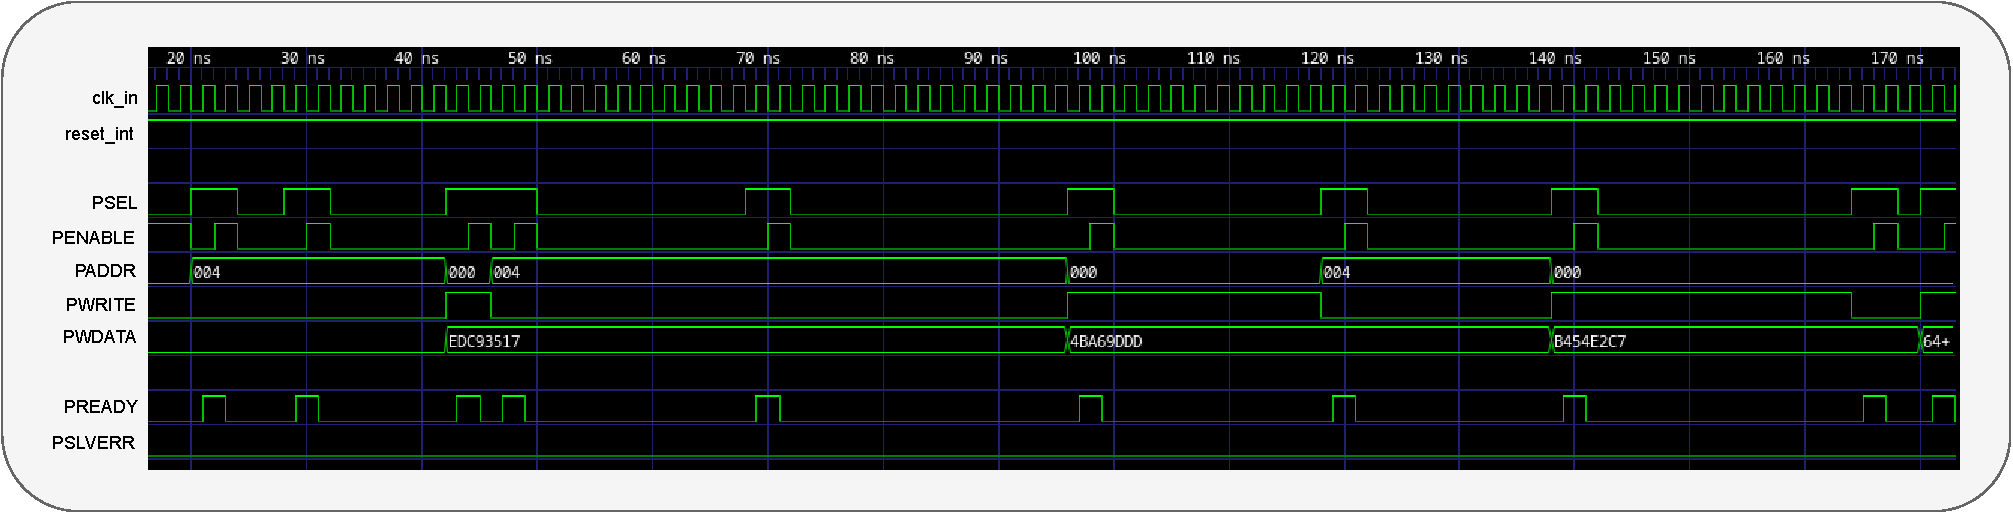
\includegraphics[width=\textwidth]{diagrams/apb_timing.pdf}
  \caption{Waveform showing the driving of 10 APB transactions with random intervals in between transactions.}
  \label{fig:apb_timing}
\end{figure}


\chapter{Discussion} %/////////////////////////////////////////////////////////////////////////////////////////////////////////


This thesis has proposed a verification framework for SystemVerilog designs implemented in Scala 3. The framework allows for multi-threaded testbenches using a peek/poke/step interface to interact with DUT. On top of the simulation interface, which facilitates the construction of unit tests, a library of standard testbench components taken from the UVM was implemented. The execution of these testbenches is structured through a simplified phasing model. Configuration and flexibility are provided through the use of compile-time safe factories for components, sequences, transactions, and configuration objects alongside a hierarchy-aware parameter system inspired by the UVM factory and configuration database.

The framework's primary interface to the simulation is influenced by the Chiseltest framework. Most importantly, a \ttt{step} interface is used to advance the simulation by whole clock cycles instead of synchronizing the simulation thread directly with clock edges. Code in the verification framework can only ever run at the falling edge of the clock. This is less flexible than what is possible in SystemVerilog and Cocotb, but it works well for sequential designs, which are the most common cases. 

One issue in the framework is handling Mealy outputs, i.e., outputs that depend on the inputs. The testbench can only see the change in value after the next clock edge because inputs are driven after simulation threads have finished their work. This should be fixed so that the view of the simulation threads accurately represents the behavior of the DUT.

One contribution of the framework is the support for multiple clocks using the \ttt{step} interface. This was not possible in the Chiseltest framework. To handle the correct driving of inputs relative to their clocks, clock domain declarations are necessary. Another improvement over Chiseltest is the ability to control the periods of clocks and the simulation time resolution. These are features that SystemVerilog and Cocotb already offer due to their lower level of timing control. One final improvement over the Chiseltest framework is the ability to read the internal state of the DUT. This feature is again also present in Cocotb and SystemVerilog. However, access to the internal state is untyped and does not allow for depositing values. This should be added to the proposed framework to fully replicate the capabilities of SystemVerilog and Cocotb.

A disadvantage of the framework is that the interface of the DUT has to be replicated from the RTL to Scala. However, since interfaces should be defined early in the design process and thus stay stable, this should not be a significant limitation.

The implementation of the framework utilizes virtual threads, a relatively new feature in the UVM, to provide lightweight concurrency. This is contrary to Chiseltest which uses normal operating system threads with more overhead. Furthermore, Chiseltest actually serializes the execution of threads, while the verification framework lets all threads released in a clock cycle run truly concurrently. This also contrasts Cocotb, where coroutines with cooperative multitasking are used. The Gears library was used to provide a set of higher-level concurrent abstractions, such as futures and channels. This is, however, not strictly necessary, and a more direct integration of the management of threads with the simulation environment might be a better solution in the long run, which allows for greater control over the management of the threads. This is especially true because all of the asynchronous functionality of the Gears library, like the \ttt{await} calls, are hidden from the user between the API of the framework.

One issue with the current implementation of the framework is that context parameters are polluting a lot of the code. This is especially the case due to the need to accept both the simulation and the Gears Async context parameter in all functions that interact with the simulation. If the Gears library was removed, the Async context parameter could be removed as well, and its functionality could be integrated into the simulation context. Having to accept one context parameter already seems like a more acceptable solution. Alternatively, the Scala context parameter system could be avoided entirely, and dynamic variables could be used instead to provide context. This is how the simulation controller is accessed in Chiseltest. This has the disadvantage that access to the simulation outside of a context that provides simulation capabilities, i.e. a test case, would cause runtime errors instead of compile time errors as in the current implementation. 

The RTL design is simulated using a Verilator model. Like in Chiseltest, native functions interacting with the C++ model are called through JNA. One advantage of this simulation approach, which Chiseltest and Cocotb share over SystemVerilog, is that simulation model compilation is decoupled from the compilation of the testbench, which means that a change in the testbench does not require a recompilation of the design source code. This is especially useful for large designs that have long compilation times. One disadvantage of implementing the simulation control in Scala is that calling native C++ code is expensive since JVM parameters have to be translated to native ones. In the simulation framework from SpinalHDL, the simulation runtime is moved to C++. Here the situation is reversed, with the C++ code calling Scala closures to execute the user code. It would be interesting to measure how this affects performance compared to the current implementation. In general, the number of calls to the native code should be limited. For instance, setting multiple inputs in one call instead of multiple could be a good optimization.

The first two use cases demonstrate the usage of the verification framework for small directed unit tests. For now, these tests are not organized in any way and provide no mechanism for grouping and labeling tests. Chiseltest integrates with the ScalaTest framework to provide this functionality, which could be added to the verification framework in the future.

The third and fourth use cases demonstrate the capability of the framework to replicate UVM testbenches. The framework ended up keeping the structure of a testbench close to that of UVM. Especially the subset of UVM presented by \citeauthor{sutherland2015uvm} \cite{sutherland2015uvm} provides a clear and relatively simple structure for testbenches. It was chosen to follow the advice of \cite{sutherland2015uvm}, which allowed for ignoring many of the more complex features of the UVM. The structure of components, sequences, and test cases establishes clear and proven interfaces between the different parts of the testbench. What this framework contributes, are simplifications in the concepts such that they are as minimal as possible while still facilitating reuse. Furthermore, the framework contributes some adjustments that make the usage of these concepts more concise and, in some cases, safer through the use of Scala's type system and meta-programming capabilities.

One of the simplified concepts is the phasing system. One contribution is the usage of traits to make phases opt-in instead of having all components include all phases by default. Focusing on the primary purpose of phases, the synchronization between multiple concurrent components, it was also argued that not all phases, especially in the build and cleanup regions, were strictly necessary. An argument was made that in this framework, the building of the testbench can be done through the constructor in one pass instead of multiple phases. Since components are completely initialized once their constructor returns, including their sub-components, it is impossible to reference uninitialized components this way. However, there is a limitation to this approach. When inheritance is used, Scala automatically calls the constructor of the base class. This can create situations where the base class constructor configures a component in a way not desired by the derived class, and that configuration would then have to be reversed in the derived class. This can become difficult if side effects are created by the base class constructor. In the UVM, the construction and configuration can be split over multiple phases such that the derived component only has to overwrite the part that is not desired. This is, however, a very specific case, and the simplification of the phasing system is generally beneficial to the framework's usability. 

The component implementations largely follow their UVM counterparts. One contribution is the addition of synchronization methods to wait for monitors and drivers based on a target transaction count. This allows a test case to wait for an expected amount of transactions to occur on a given interface. The provided sequencer implementation differs from that of the UVM. Instead of arbitrating access to the driver on a per-transaction basis, the sequencer plays one complete sequence at a time. This simplification works well for simple cases, but it is impossible to mix transaction streams. The framework does not address the concept of virtual sequencers either. Both issues should be investigated in the future. 

The sequences in the framework allow for the creation of transaction streams based on a feedback stream of transactions just like in UVM. However, a series of composition mechanisms are contributed to increase the usability of sequences. Instead of just sending one item and receiving one response, a sequence can directly play another sequence without creating a virtual sequence. In addition, standard composition operations such as concatenation, mixing, or repetition of sequences are provided. Finally, the framework also allows for using Scala collections to build non-feedback stimuli streams. This can be useful when the relation between transactions in the stream is simple and no feedback from the driver is needed. Virtual sequences that target different sequencers, like they can be found in the UVM, have not been investigated. This could be a future improvement.

The configuration system in the framework is inspired by the UVM factory and configuration database but adapts them to Scala's capabilities. The framework provides factories for each testbench ground type - components, sequences, transactions, and configuration objects. Although the UVM factory allows for the creation of general UVM objects through one factory, these four factories cover the most common use cases where a factory is needed to change out implementations. The splitting of the factory is necessary to create compile-time safe interfaces. This contribution means that all factory override and creation calls check at compile time that only classes with the correct type and constructor will be created and that only derived classes with the correct constructor override their supertype. 

The configuration context consists of factory overrides and key-value parameters that are inherited through the hierarchy, just like in UVM. However, it is avoided to use hierarchical string paths to define the scope of a configuration. Instead, the configuration is passed through the factory call to the component, sequence, or transaction that is created. The context builder allows for the creation of a configuration context that can be reused to create multiple instances. The interface to the key-value configuration parameters was improved to include option return types and default values to make handling missing parameters easier. 

One feature this factory implementation does not support is the ability to override a type from the command line, as it is possible in UVM. In UVM, the test case that should be executed is also defined in the command line, such that only one compilation is needed for all tests. Scala, however, supports multiple entry points to a program. As such, one entry point should be dedicated to each test case which should define its specific overrides. This is the only way to give the compile-time guarantees that all factory calls and overrides will work since it means that all overrides are statically known.


The goal of the project was to explore how the integration of a verification framework with the concepts of the UVM would benefit from a modern high-level language such as Scala. The four use cases show that the framework is generally capable of implementing some small verification tasks. The comparison with the PyUVM test case in use case 3 showed that the framework's contributions have an impact on the conciseness of the testbench code, even in such a simple case. It showed that the framework is capable of replicating the test case even though some UVM concepts were simplified or removed. The first two use cases demonstrate how small directed test cases can be easily created that do not use any verification components and are not subject to phasing. For these types of tests, the framework thus matches the capabilities of Chiseltest, except for the lack of integration with ScalaTest. In the third use case, it was possible to match the capabilities of a PyUVM testbench. The PyUVM implementation of the APB verification infrastructure was more complex and not fully replicated due to time constraints. The aspects that were not replicated relate however mostly to the configurability of the APB agent for different bus widths and for taking the producer or consumer role. This behavior is expected to be replicable in the proposed framework since it does not require any mechanisms specific to UVM but relies on general language features.

Generally, it can be seen that the simplifications made to the UVM also can cause some limitations in particular cases. One of the problems of designing a framework is the anticipation of \textit{how} it might be used. This is a challenging task for infrastructure meant for complex systems. Many of the mechanisms of the UVM do not make sense on a small scale but instead bear fruit when used in large projects. Designing such a framework requires real-world experience with large verification projects to judge what limitations are, in the end, acceptable and which are not. As such, the framework should be seen as a starting point, trying to formulate a minimal subset with an API tailored to simplicity. Taking this as a basis, the framework could be extended to include more complex features.

One very binding design choice is the language, which in this framework was Scala 3. Since the aim was to explore hardware verification in a modern language, the newest language features should be used and as such also the newest version of a language. This, however, limits the integration with existing Scala solutions at the current point. All Chisel and Chiseltest infrastructure are far away from achieving compatibility with Scala 3. Since a Scala verification framework would be more useful if used together with Chisel, this is a notable limitation.

The proposed framework can be seen as a proof of concept showing the potential of using a modern high-level language for verification and tailoring the framework to the language. This framework can therefore be seen as the starting point for further exploration. Several smaller features that the UVM offers, such as transaction recording, still have to be investigated since they are necessary for certain verification tasks. Most importantly, the framework should however be evaluated on larger and more complex designs to see how well the simplifications hold up at that scale. To make the framework a credible alternative, its performance should be evaluated and compared to existing solutions like Cocotb but also UVM testbenches running on commercial simulators.

\chapter{Conclusion} %/////////////////////////////////////////////////////////////////////////////////////////////////////////

This thesis explored the adaptation of the Universal Verification Methodology (UVM) principles to a modern high-level programming language, specifically Scala 3. Through three interviews and an investigation of current verification frameworks and the UVM, a verification framework was proposed. The goal was to bring a core subset of composability and reusability concepts for testbenches from the UVM into a verification environment inspired by existing testing frameworks in high-level languages such as Cocotb and Chiseltest. The implemented multi-threaded simulation interface extends the peek/poke/step interface of Chiseltest to work with multiple clock domains. The proposed framework takes advantage of Scala's advanced features, such as strong type safety and meta-programming to enable concise testbench descriptions and to offer compile-time safety whenever possible, such as in the case of the factory. Other key contributions include a simplified phasing and component system as well as a more powerful sequence system that facilitates the mixing of UVM-like sequences and Scala sequences. The reduction to a minimal set of features and the simplification of these make the proposed framework more approachable while still maintaining the core verification capabilities of the UVM. 

To evaluate the framework, multiple use cases were implemented, including replicating a PyUVM testbench for a small ALU design and implementing part of the verification infrastructure for APB interfaces for the Didactic SoC. These use cases demonstrated that the framework is capable of supporting various verification scenarios with a slight reduction in complexity in a direct comparison with PyUVM.

While the framework offers a promising alternative, it also has some limitations. The simplification of the construction phase of the testbench makes the initialization of components safer, but it may also limit how derived components can overwrite their ancestor's behavior. The simulation interface provides a simple way of controlling the DUT but has an issue with Mealy outputs in its current implementation. Finally, while implementing the framework in Scala 3 allowed for leveraging modern language features, it currently limits integration with existing Scala solutions such as Chisel and ChiselTest, which only support Scala 2.

The framework serves as a proof of concept that showcases the potential of using a modern high-level language for verification. Future work should focus on further validation of the framework through larger and more complex use cases to see how the simplifications perform at a larger scale. Furthermore, the performance should be evaluated against industry-standard solutions such as Cocotb/PyUVM and commercial UVM testbenches.


